\documentclass[12pt]{report}
%\usepackage{amsfonts}
%\usepackage{graphics}
%\usepackage[round,authoryear]{natbib}
\usepackage{rotating}
\usepackage{tocloft}
\usepackage{color}
%\usepackage{fancyhdr}
\usepackage{amsmath}
\usepackage{amsfonts}
%\usepackage{url}
\usepackage{subfig}
\usepackage{hyperref}
\usepackage{textcomp}
\usepackage{verbatim}
\newcommand{\micron}{\textmu{}m} 
\newcommand{\Finesse}{$\mathcal{F}$}

\newcommand{\half}{\frac{1}{2}}
\newcommand{\threehalf}{\frac{3}{2}}
\newcommand{\regh}{\mathfrak{h}}
\newcommand{\bfrho}{\mbox{\boldmath$\rho$}}
\newcommand{\bfh}{\mbox{\boldmath$\mathfrak{h}$}}
\renewcommand{\cftchapdotsep}{\cftdotsep}
\usepackage{setspace}
%\usepackage{fullpage}
%%%%%%%%%%%%%%%%%%%%%%%%%%%%%%%%%%%%%%%%%%%%%%%%%%%%%%%%%%%%%%%%%%%%%%%%%%%
%
%				COMMANDS
%
% \singlespace     = start single spacing (0.165in between lines)
% \doublespace     = start double spacing (0.330in between lines)
% \CHAPTER{}       = chapter heading
% \TOPPER{}        = heading for such things as Acknowledgments, TOC, etc.
% \APPENDIX{}      = appendix header
% \SECTION{}       = section header
% \SUBSECTION{}    = subsection header
% \SUBSUBSECTION{} = subsubsection header
%
% The left hand margin is set up for 1.5 inches, and the text length is
% set up for 9 inches.  Extra space above and below the equations is
% removed.
%
%%%%%%%%%%%%%%%%%%%%%%%%%%%%%%%%%%%%%%%%%%%%%%%%%%%%%%%%%%%%%%%%%%%%%%%%%%%
\newcommand{\singlespace}{\setlength{\baselineskip}{0.165in}}
\newcommand{\doublespace}{\setlength{\baselineskip}{0.33in}}
\newcommand{\hi}{H I}
% Print out...
%\setlength{\oddsidemargin}{0.75in}
%
% Online submission
\setlength{\oddsidemargin}{0.0in}
%\setlength{\textheight}{7.5in} - I added
\setlength{\topmargin}{-1cm}
%\setlength{\textheight}{8.5in} original
\setlength{\textheight}{8.5in}
\setlength{\textwidth}{6.5in}
\addtolength{\abovedisplayskip}{-1em}
\addtolength{\abovedisplayshortskip}{-1em}
\pagestyle{myheadings}

\newcommand{\CHAPTER}[1]{%
\refstepcounter{chapter}%
\addcontentsline{toc}{chapter}{\thechapter . #1}%
%%\addcontentsline{toc}{chapter}{\protect\numberline{\thechapter}#1}%
\newpage%
\pagestyle{myheadings}
\thispagestyle{plain}%
\singlespace%
\begin{center}% 
%%\textbf{CHAPTER~\thechapter}\\%
%%\textbf{\thechapter}\\%
\LARGE
\textbf{\thechapter}%
%%\vspace{2em}%
\textbf{. #1}\\%
\normalsize
\end{center}%
\doublespace%
\vspace{2em}
\singlespace}


\newcommand{\TOPPER}[1]{%
\addcontentsline{toc}{chapter}{#1}%
\newpage%
\pagestyle{plain}%
\begin{center}% 
\LARGE
\textbf{#1}\\%
\normalsize
\end{center}%
\vspace{2em}
\singlespace}

\newcommand{\NOTOPPER}[1]{%
\addcontentsline{toc}{chapter}{#1}%
\newpage%
\pagestyle{plain}%
\vspace{2em}%
\singlespace}

\newcommand{\REFVIT}[1]{%
\newpage%
\thispagestyle{plain}%
\begin{center}% 
\textbf{#1}\\%
\end{center}%
\vspace{2em}}

\newcommand{\APPENDIX}[1]{%
\refstepcounter{chapter}%
\addcontentsline{toc}{chapter}{\protect\numberline{\thechapter}}%
\newpage%
\pagestyle{myheadings}
\thispagestyle{plain}%
\singlespace%
\begin{center}% 
\LARGE
\textbf{APPENDIX A: #1}\\%
%%\textbf{APPENDIX~\thechapter: #1}\\%
%%\vspace{2em}%
%%\textbf{#1}\\%
\normalsize
\end{center}%
\doublespace%
\vspace{2em}}

\newcommand{\SECTION}[1]{%
\refstepcounter{section}%
\addcontentsline{toc}{section}{\protect\numberline{\thesection}#1}%
{\vspace{1em} \noindent \Large \textbf{\thesection~#1}\par \normalsize \vspace{1em}}}

\newcommand{\SUBSECTION}[1]{%
\refstepcounter{subsection}%
\addcontentsline{toc}{subsection}{\protect\numberline{\thesubsection}#1}%
{\vspace{1em} \noindent \normalsize \textbf{\thesubsection~#1}\par \vspace{1em}}}

\newcommand{\SUBSUBSECTION}[1]{%
\refstepcounter{subsubsection}%
\addcontentsline{toc}{subsubsection}{\protect\numberline{\thesubsubsection}#1}%
{\vspace{1em} \noindent \normalsize \textbf{\thesubsubsection~#1}\par \vspace{1em}}}

\def\contentsname{\normalsize \centerline{\textbf{TABLE OF CONTENTS}}}%

\newcommand{\gtrsim}{\mathrel{\hbox{\rlap{\hbox{\lower4pt\hbox{$\sim$}}}\hbox{$>$}}}}
\newcommand{\lesssim}{\mathrel{\hbox{\rlap{\hbox{\lower4pt\hbox{$\sim$}}}\hbox{$<$}}}}
\newcommand{\sq}{\hbox{\rlap{$\sqcap$}$\sqcup$}}
\newcommand{\arcdeg}{\hbox{$^\circ$}}
\newcommand{\arcmin}{\hbox{$^\prime$}}
\newcommand{\arcsec}{\hbox{$^{\prime\prime}$}}
\newcommand{\sun}{\hbox{$\odot$}}
\newcommand{\earth}{\hbox{$\oplus$}}

%% FIX THE G_DAMN TABLE OF CONTENTS SO THE FONTS ARE ALL THE SAME FREAKING SIZE
\renewcommand{\cftchapfont}{\normalfont}

%% And make sure the page numbers are all the same font...
\renewcommand{\cftchappagefont}{\normalfont}

%% Make the dots the same size regardless of entry type
\renewcommand{\cftdot}{\normalfont.}


%% Need to do this to trick LaTeX into setting the Bibliography closer to
%% what TOPPER does.
\renewcommand{\bibname}{\vspace{-0.9in} \begin{center} \LARGE \textbf{Bibliography} \normalsize \end{center}}
%\setlength{\oddsidemargin}{0.2in}
%\setlength{\evensidemargin}{0in}
%\setlength{\topmargin}{0.8in}
%%\setlength{\textheight}{9in}
%\setlength{\textwidth}{6in}
%\setlength{\headheight}{0.0in}
%\setlength{\headsep}{0.2in}
%%%%%%%%%%%%%%%%%%%%%%%%%%%%%%%%%%%%%%%%%%%%%%%%%%%%%%%%%%%%%%%%%%%%%%%%%%%%%
%
%				COMMANDS
%
% \singlespace     = start single spacing (0.165in between lines)
% \doublespace     = start double spacing (0.330in between lines)
% \CHAPTER{}       = chapter heading
% \TOPPER{}        = heading for such things as Acknowledgments, TOC, etc.
% \APPENDIX{}      = appendix header
% \SECTION{}       = section header
% \SUBSECTION{}    = subsection header
% \SUBSUBSECTION{} = subsubsection header
%
% The left hand margin is set up for 1.5 inches, and the text length is
% set up for 9 inches.  Extra space above and below the equations is
% removed.
%
%%%%%%%%%%%%%%%%%%%%%%%%%%%%%%%%%%%%%%%%%%%%%%%%%%%%%%%%%%%%%%%%%%%%%%%%%%%
\newcommand{\singlespace}{\setlength{\baselineskip}{0.165in}}
\newcommand{\doublespace}{\setlength{\baselineskip}{0.33in}}
\newcommand{\hi}{H I}
% Print out...
%\setlength{\oddsidemargin}{0.75in}
%
% Online submission
\setlength{\oddsidemargin}{0.0in}
%\setlength{\textheight}{7.5in} - I added
\setlength{\topmargin}{-1cm}
%\setlength{\textheight}{8.5in} original
\setlength{\textheight}{8.5in}
\setlength{\textwidth}{6.5in}
\addtolength{\abovedisplayskip}{-1em}
\addtolength{\abovedisplayshortskip}{-1em}
\pagestyle{myheadings}

\newcommand{\CHAPTER}[1]{%
\refstepcounter{chapter}%
\addcontentsline{toc}{chapter}{\thechapter . #1}%
%%\addcontentsline{toc}{chapter}{\protect\numberline{\thechapter}#1}%
\newpage%
\pagestyle{myheadings}
\thispagestyle{plain}%
\singlespace%
\begin{center}% 
%%\textbf{CHAPTER~\thechapter}\\%
%%\textbf{\thechapter}\\%
\LARGE
\textbf{\thechapter}%
%%\vspace{2em}%
\textbf{. #1}\\%
\normalsize
\end{center}%
\doublespace%
\vspace{2em}
\singlespace}


\newcommand{\TOPPER}[1]{%
\addcontentsline{toc}{chapter}{#1}%
\newpage%
\pagestyle{plain}%
\begin{center}% 
\LARGE
\textbf{#1}\\%
\normalsize
\end{center}%
\vspace{2em}
\singlespace}

\newcommand{\NOTOPPER}[1]{%
\addcontentsline{toc}{chapter}{#1}%
\newpage%
\pagestyle{plain}%
\vspace{2em}%
\singlespace}

\newcommand{\REFVIT}[1]{%
\newpage%
\thispagestyle{plain}%
\begin{center}% 
\textbf{#1}\\%
\end{center}%
\vspace{2em}}

\newcommand{\APPENDIX}[1]{%
\refstepcounter{chapter}%
\addcontentsline{toc}{chapter}{\protect\numberline{\thechapter}}%
\newpage%
\pagestyle{myheadings}
\thispagestyle{plain}%
\singlespace%
\begin{center}% 
\LARGE
\textbf{APPENDIX A: #1}\\%
%%\textbf{APPENDIX~\thechapter: #1}\\%
%%\vspace{2em}%
%%\textbf{#1}\\%
\normalsize
\end{center}%
\doublespace%
\vspace{2em}}

\newcommand{\SECTION}[1]{%
\refstepcounter{section}%
\addcontentsline{toc}{section}{\protect\numberline{\thesection}#1}%
{\vspace{1em} \noindent \Large \textbf{\thesection~#1}\par \normalsize \vspace{1em}}}

\newcommand{\SUBSECTION}[1]{%
\refstepcounter{subsection}%
\addcontentsline{toc}{subsection}{\protect\numberline{\thesubsection}#1}%
{\vspace{1em} \noindent \normalsize \textbf{\thesubsection~#1}\par \vspace{1em}}}

\newcommand{\SUBSUBSECTION}[1]{%
\refstepcounter{subsubsection}%
\addcontentsline{toc}{subsubsection}{\protect\numberline{\thesubsubsection}#1}%
{\vspace{1em} \noindent \normalsize \textbf{\thesubsubsection~#1}\par \vspace{1em}}}

\def\contentsname{\normalsize \centerline{\textbf{TABLE OF CONTENTS}}}%

\newcommand{\gtrsim}{\mathrel{\hbox{\rlap{\hbox{\lower4pt\hbox{$\sim$}}}\hbox{$>$}}}}
\newcommand{\lesssim}{\mathrel{\hbox{\rlap{\hbox{\lower4pt\hbox{$\sim$}}}\hbox{$<$}}}}
\newcommand{\sq}{\hbox{\rlap{$\sqcap$}$\sqcup$}}
\newcommand{\arcdeg}{\hbox{$^\circ$}}
\newcommand{\arcmin}{\hbox{$^\prime$}}
\newcommand{\arcsec}{\hbox{$^{\prime\prime}$}}
\newcommand{\sun}{\hbox{$\odot$}}
\newcommand{\earth}{\hbox{$\oplus$}}

%% FIX THE G_DAMN TABLE OF CONTENTS SO THE FONTS ARE ALL THE SAME FREAKING SIZE
\renewcommand{\cftchapfont}{\normalfont}

%% And make sure the page numbers are all the same font...
\renewcommand{\cftchappagefont}{\normalfont}

%% Make the dots the same size regardless of entry type
\renewcommand{\cftdot}{\normalfont.}



\begin{document}
\pagenumbering{roman}
\thispagestyle{empty}
%\begin{titlepage}
\begin{center}
\textbf{DC Readout in Enhanced LIGO}
\vspace{1.75in}

A Dissertation\\
\vspace{1ex}
Submitted to the Graduate Faculty of the\\
Louisiana State University and\\
Agricultural and Mechanical College\\
in partial fulfillment of the\\
requirements for the degree of\\
Doctor of Philosophy\\
\vspace{1ex}
in\\
\vspace{1ex}
The Department of Physics and Astronomy\\
\vspace{1in}
\texttt{\color{red}{DRAFT compiled \today}}
\vspace{0.75in}

by\\
Tobin Thomas Fricke \\
B.S., University of California, Berkeley, 2003\\
M.A., University of Rochester, 2005 \\

\begin{tabular}{c}
\\
\\
\\
\\
\\
August 2011
\end{tabular}

\end{center}


\chapter*{}  % Dedication page should have no title.
\doublespace
For my parents, who have always supported and encouraged me.
  

\singlespace
\NOTOPPER{Acknowledgements}
\chapter*{Acknowledgements}

It has been a privilege to be a part of the nascent field of
gravitational wave astronomy at this exciting time, perhaps at the
cusp before an era of discovery.  It would be impossible to properly
acknowledge all of the great people I have encountered and who have
influenced me during my time in graduate school, but I will nonetheless
try to name the main characters.

Thank you to Adrian Melissinos, my advisor at the University of
Rochester, for your energy and creativity, and for getting me involved
with gravitational waves in the first place.  

To Rana Adhikari, my mentor at Caltech and a driving force behind
Enhanced LIGO, for showing me how to align the mode cleaner and cut
the can off of photodiodes.
%, solder
%tiny parts, and brew acceptable coffee.

To Valery Frolov at LIGO Livingston, a tireless commissioner and
uncompromising scientist, for mentoring me and for countless late
night hours in the control room.

To Gabriela Gonz\'alez, my advisor at Louisiana State University, for
adopting me as a student and guiding me through the graduate school
process with the utmost patience, and for letting us drink Jorge's
whiskey.

And to Rai Weiss, a role model for us all.

Thank you also to my fellow graduate students and friends, among them
Kate Dooley, Stefanos Giampanis, Ryan Dahl, Lisa Togler, Kris Yirak,
Aimee Slaughter, Bree Lupia, Matthew Bryant, and Sara DeRosier.  To
my cohort at LSU: Anamaria Effler, Ryan DeRosa, Chad Hanna, Jeff
Kissel, Jake Slutsky, Rupal Amin, and Sarah Caudhill.  To Rob Ward,
Marie-H\'el\`ene, Jeff Smith, Dan Busby, Phil Willems, Steve Vass, and
John Miller for making my stay at Caltech an enjoyable one.  And to
everyone else who worked on the Enhanced LIGO project or continues to
work towards the detection of graviational waves.

%\NOTOPPER{Preface}
%\chapter*{Preface}

Finally, the boilerplate: this work was supported by the National
Science Foundation under grant
\href{http://www.nsf.gov/awardsearch/showAward.do?AwardNumber=0905184}{PHY-0905184}.
LIGO was constructed by the California Institute of Technology and
Massachusetts Institute of Technology with funding from the National
Science Foundation and operates under cooperative agreement
\href{http://www.nsf.gov/awardsearch/showAward.do?AwardNumber=0757058}{PHY-0757058}.
This dissertation has LIGO Document number LIGO-P1000010.



\singlespace
\tableofcontents


\clearpage
\singlespace
\NOTOPPER{List of Tables}
\doublespace
\listoftables


\clearpage
\singlespace
\NOTOPPER{Figures}
\listoffigures


\clearpage
\singlespace
\chapter*{Abstract}
%% The abstract is a brief description of your research project. It
%% should describe the problem being addressed, how you addressed it,
%% the results and conclusions reached.  The abstract may not contain
%% graphs, tables or illustrations. An English translation should be 
%% provided of an abstract in a foreign language.  The abstract must be
%% no more than 350 words, counting enumerations, numerals, articles,
%% and components of hyphenated compounds as one word each.  The line
%% spacing of the abstract should be the same as that chosen for the
%% text.  
Gravitational waves are ripples of space-time predicted by Einstein's
theory of General Relativity.  The Laser Interferometer
Gravitational-wave Observatory (LIGO), part of a global network of
gravitational wave detectors, seeks to detect these waves and study
their sources.

The LIGO detectors were recently upgraded with the dual goals of
increasing the sensitivity (and liklihood of detection) and proving
techniques for Advanced LIGO, a major upgrade currently underway.  As
part of this upgrade, the signal extraction technique was changed from
a heterodyne scheme to a form of homodyne detection called DC readout.
The DC readout system includes a new optical filter cavity, the output
mode cleaner, which removes unwanted optical fields at the
interferometer output port.

This work describes the implementation and characterization of the new
DC readout system and output mode cleaner, including the achieved
sensitivity, noise couplings, and servo control systems.

%% for word count:
%% grep --invert-match "^%%" abstract.tex | wc --words

\pagenumbering{arabic}
\clubpenalty=10000
\widowpenalty=10000

\pagestyle{myheadings}

\CHAPTER{Introduction}
\label{chapter1}
\doublespace

\SECTION{Gravitational Waves}

Almost all of humanity's knowledge of the universe is derived from
observations of electromagnetic waves.  The effort to detect
gravitational waves seeks to expand this knowledge by observing an
entirely different field, and to further verify the correctness of the
theory of general relativity.

Any theory of gravity that avoids instantaneous action at a distance
must feature some kind of gravitational waves.  Even Newtonian gravity
can be modified to account for propagation delays from massive bodies
that are the sources of attraction\cite{Schutz1984Gravitational}.
Gravity as we know it, however, is described by the general theory of
relativity.  In general relativity, spacetime is treated as a
four-dimensional manifold with some intrinsic curvature.  This
curvature is generated by the presense of mass and energy.  In the
absense of forces, particles follow geodesic trajectories on this
manifold.  Thus, in the quintessential words of John Wheeler(?),
``Space tells matter how to move, matter tells space how to curve.''

This relationship between matter and curvature is made formal through
the Einstein field equation, which equates (up to units) the Einstein
tensor ($\mathsf{G}$), encoding curvature, with the
Stress-Energy tensor ($\mathsf{T}$), encoding the matter and energy
contents:
\begin{equation}
\mathsf{G} = \frac {8\pi G}{c^4} \mathsf{T}
\end{equation}
where $G$ is (Newton's) universal gravitational constant and $c$ is
the speed of light.

To perform calculations, we typically need to work in some coordinate
basis.  Thus one will work with $G_{\mu\nu}$, where $\mu$ and $\nu \in
{0,1,2,3}$ are coordinate indices.  In this notation, the Einstein
tensor is givenby $G_{\mu\nu} = R_{\mu\nu} - \frac{1}{2} R
g_{\mu\nu}$, where $R_{\mu\nu}$ is the Ricci curvature tensor, $R$ is
the Ricci scalar, and $g_{\mu\nu}$ is the spacetime metric.  The
metric plays a central role here, as it both encodes the curvature and
implicitly defines the coordinate system.

\begin{figure}
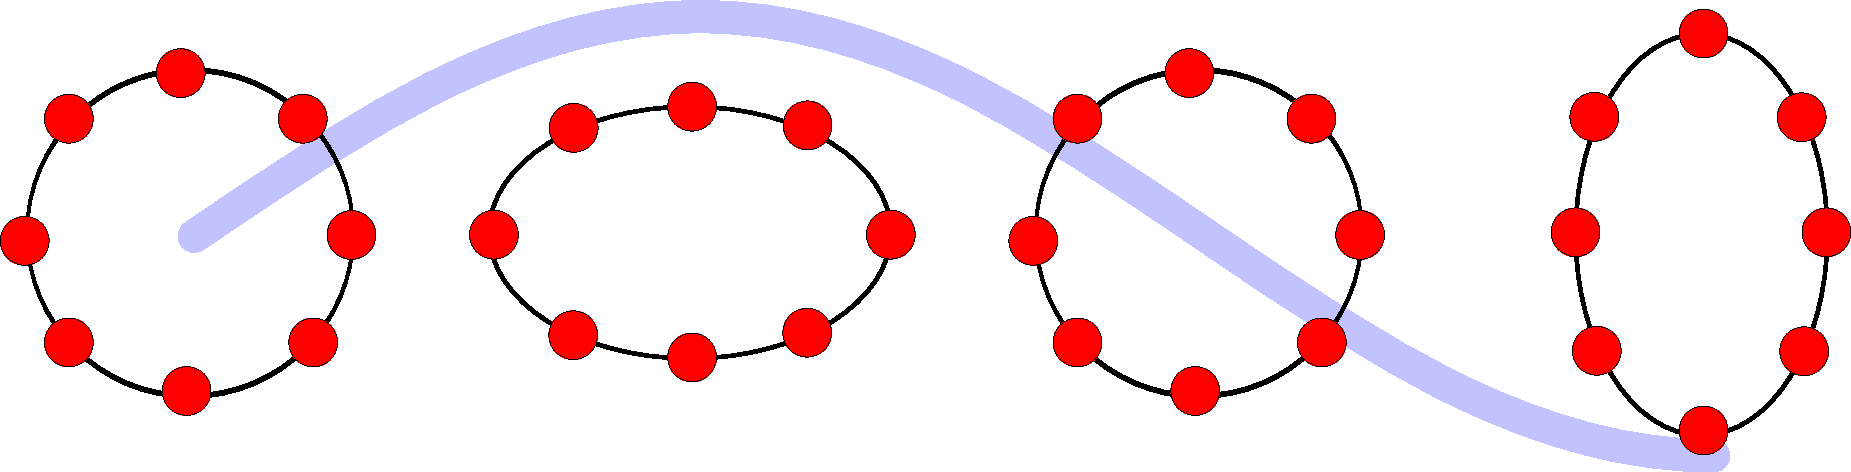
\includegraphics[width=\columnwidth]{chapter1/figures/gwave.pdf}
\caption{\label{fig:gwave-effect}Depiction of the effect of a
  gravitational wave (traveling into the page) on a ring of
  non-interacting inertial test particles.}
\end{figure}

To reveal the mechanism of gravitational waves, we are interested in
vacuum ($\mathsf{T}=0$) solutions of the Einstein field equations in
the weak-field limit.  In the weak-field limit, we can write the
metric $g_{\mu\nu}$ as the sum of the flat-space Minkowski metric
$\eta_{\mu\nu}$ and a small perturbation $h_{\mu\nu}$:
$$g_{\mu\nu} = \eta_{\mu\nu} + h_{\mu\nu}$$ This is the regime of
linearized gravity.  Calculating out the Einstein field equation
keeping only terms of first-order in $h$ and choosing the
transverse-traceless gauge, one finds (see Sean Carroll's lucid
exposition in \cite{Carroll1997Lecture} for the details) a wave
equation for $h$:
$$\left(\nabla^2 - \frac{1}{c^2}\frac{\partial^2}{\partial t^2}\right)h_{\mu\nu} = 0$$
where $h_{\mu\nu}$ has, for a wave propagating along the $z$ axis, the form:
$$ [\mathsf{h}] = \left(
\begin{array}{cccc}
0 & 0 &  0 & 0 \\
0 & a &  b & 0 \\
0 & b & -a & 0 \\ 
0 & 0 &  0 & 0 
\end{array}
 \right)$$
Here we see several of the essential points of gravitational waves:
\begin{itemize}
\item There are two independent components (polarizations)
\item They travel at the speed of light 
\item They are manifest as a transverse tidal force on inertial objects
\end{itemize}

The amplitude of gravitational waves is quantified as the effective
strain exerted on inertial test-masses.

\SECTION{The Hulse-Taylor Pulsar}

Gravitational waves have not yet been directly detected, but very
strong indirect evidence exists.  Perhaps the strongest evidence is
the Hulse-Taylor
pulsar~\cite{Hulse1975Discovery,Weisberg2005Relativistic}--a
remarkable discovery of a binary star system in which one of the
constituents is pulsar PSR B1913+16. The binary system is expected to
radiate energy away into gravitational waves, causing its orbit to
decay.  The pulsar reveals the orbital parameters of the binary
system, in particular its orbital period. Measurement of the orbital
period through pulsar tracking over 30 years shows that the orbit is
decaying exactly as predicted by general relativity.

Another binary system containing pulsars was discovered in 2004.  In
this system \emph{both} objects are
pulsars. \cite{Lyne2004DoublePulsar,Kramer2006Tests}

\SECTION{Sources of Gravitational Waves}
Any system of mass accelerating in the quadrupolar or higher moments
will radiate energy into gravitational waves.  The effect is so weak,
however, that only some of the universe's more cataclysmic events have
a chance of producing waves observable on earth.

Anticipated sources of gravitational waves can be conveniently
categorized as \emph{continuous} or \emph{transient}, and as
\emph{modeled} or \emph{unmodeled}.  There is some overlap in this
division.  Sources are paired with associated search efforts.

\begin{itemize}

\item \textbf{compact binary coalescence} --- Pairs of compact objects
  (black holes or neutron stars) in binary orbits are expected to lose
  energy through gravitational waves, causing the orbit to decay until
  the objects finally begin to interact and merge into a single
  object.  This inspiral process will generate a characteristic chirp
  signal, followed by the complex merger process and then ringdown.

\item \textbf{continuous wave} --- Rapidly spinning objects will
  generate essentially monochromatic signals, which are in turn
  doppler-shifted by the relative motion of the Earth and the source.
  This is sometimes called the pulsar search, since the primary source
  in this category is expected to be rapidly spinning neutron stars
  (such as pulsars).  The search, in turn, is divided into searches
  for known pulsars and unknown pulsars.  Pulsars which are known
  electromagnetically can be targetted directly, whereas unknown
  pulsars require a brute-force search of the parameter space.

  Currently this is attacked in part through the distributed computing
  project Einstein@Home.  One nicety of the pulsar search is that the
  process works equally well for analyzing radio telescope data--this
  has been done, resulting in the discovery of several previously
  unknown radio pulsars\cite{Knispel2010Pulsar}.  It is an open
  problem to find a more efficient search algorithm.

\item \textbf{bursts} --- Transient cataclysmic events such as
  supernovae will generate bursts of gravitational waves whose
  waveforms is not known in advance.  

\item \textbf{stochastic background} --- In the same manner as the
  cosmic microwave background radiation, a cosmological background of
  gravitational waves is expected to exist.  This is perhaps the most
  exotic anticipated source of gravitational waves, since its
  detection will inform us of the state of the universe at an age far
  earlier than has yet been probed.  Sadly, the cosmological
  background is almost certainly too weak to detect in the forseeable
  future.

  The cacophony of unresolved astrophysical sources will also combine
  to produce a gravitational wave stochastic background.   

  The stochastic background search is fully coherent.  In its simplest
  form, the search simply computes the correlation between pairs of
  gravitational wave detectors.  This can be done in either an all-sky
  search or in a sky-position-dependent search.  Typically, some
  power-law gravitational wave spectrum is assumed.

\end{itemize}

Improvements in search sensitivity can be achieved by incorporating
knowledge of the expected signal waveform or spectrum; integrating
over a long period of time (for continuous sources); and by looking
for coincidence or coherence between multiple detectors.

The global network of gravitational wave detectors is operated as a
sensor array, an interferometer composed of many interferometers.

\SECTION{Detectors}
Gravitational waves couple to both light and matter.

\begin{figure}
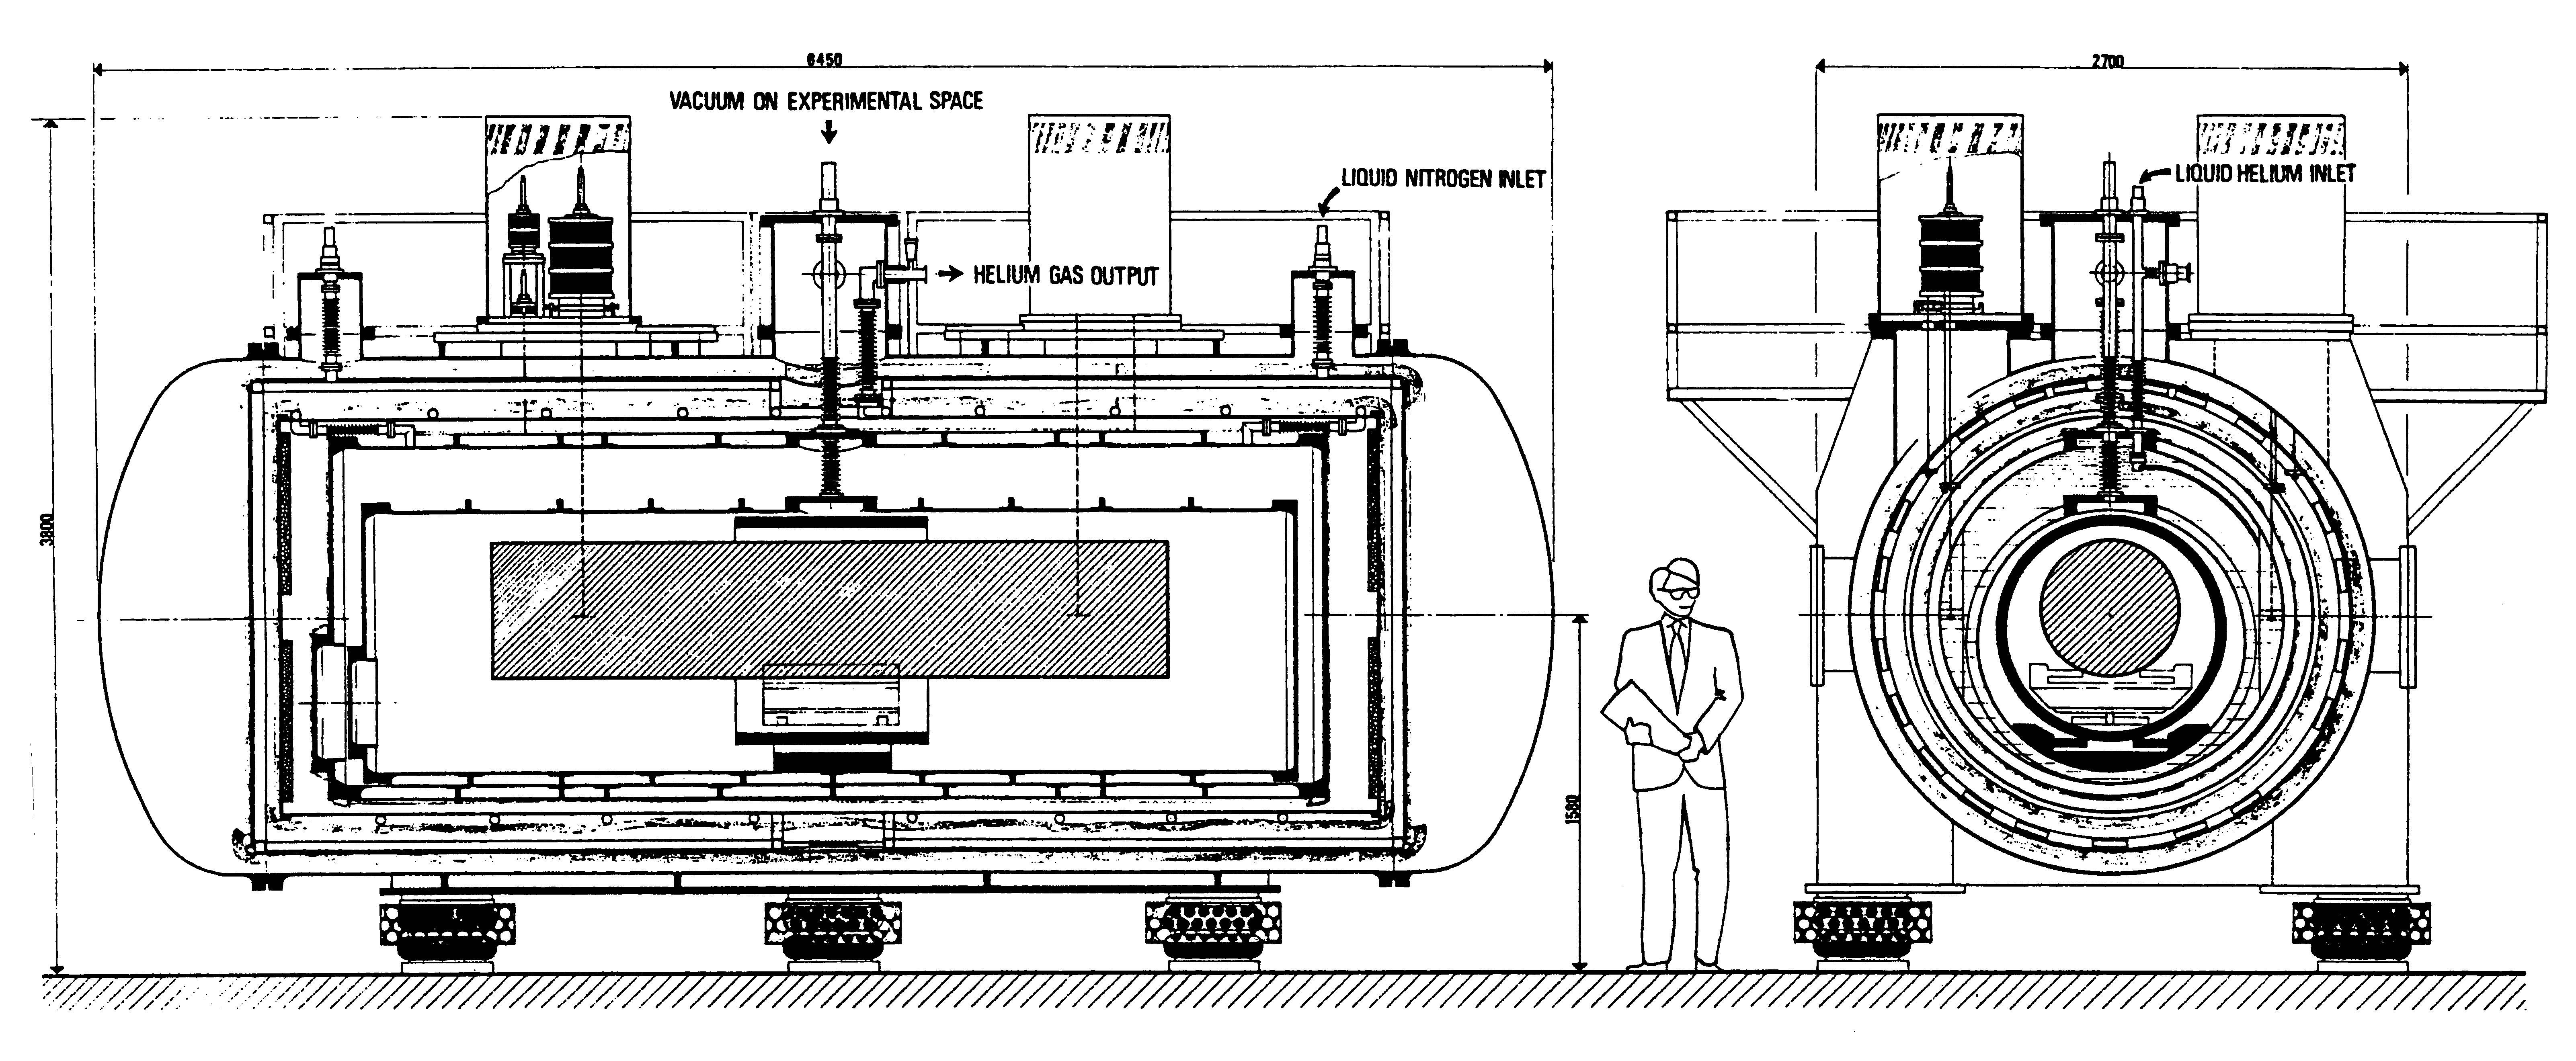
\includegraphics[width=\columnwidth]{chapter1/figures/explorer.png}
\caption{\label{fig:explorer-bar}Depiction of the cryostat of the
  EXPLORER bar detector, which operated \checkme{somewhere} for
  \checkme{some time}.  Illustration adapted from \checkme{a
    reference}.}
\end{figure}

The first attempts to detect gravitational waves used resonant bar
detectors.  In such a detector, a large cylinder of a metal alloy with
a very high mechanical Q-factor is suspended in a vacuum chamber and
cooled to cryogenic temperatures.  A passing gravitational wave
couples mechanical energy into the bar, ringing up the fundamental
mechanical mode of the bar.  Sensitive detectors (latter bars used
SQUIDs) read out this mechanical displacement.  Resonant bars are
inherently narrow-band devices, sensitive to gravitational waves
within a narrow linewidth about their fundamental resonance.

Bar detectors do have the advantage that they are small enough that
they can be moved or re-oriented.  The ALLEGRO bar detector at LSU was
once rotated to modulate its overlap function with the nearby LIGO
Livingston observatory.

\SUBSECTION{Laser interferometers}

Laser interferometers are now the instrument of choice in the search
for gravitational waves.  A gravitational wave will modulate the
optical path length of light traveling transversely through it between
inertial test masses.  This path length modulation can be detected by
a laser interferometer.  The operation of laser interferometer
gravitational wave detectors is the focus of this work and is detailed
in the following chapters.

In terrestrial interferometers, large\footnote{10 kg in Initial LIGO,
  40 kg in Advanced LIGO} glass cylinders serve as both super-polished
mirrors and inertial test masses.  These optics are hung as pendula to
allow inertial freedom of the pendular resonance frequency.

References to cite in this section: \cite{Weiss1972Electromagnetically,Forward1978Wideband}

\SUBSECTION{Other detectors}

There are a few other mechanisms by which gravitational waves may be
detected.

Pulsars serve as extremely reliable clocks, beaming a sequence of
pulses towards earth whose arrival times can typically be predicted to
better than a microsecond.  The path of the electromagnetic waves
traveling from the pulsar to earth acts in some ways like an arm of a
laser interferometer: gravitational waves passing transversely to the
Earth-Pulsar baseline will modulate the optical path length, producing
perturbations in the arrival time of the pulsar pulses--perturbations
which are correlated between observations of distinct pulsars. Pulsar
timing arrays seek to analyze these correlated residuals to find
evidence of gravitational waves;
Hobbs~\cite{Hobbs2009International} anticipates that pulsar timing
analysis will yield detections of gravitational waves in the nanohertz
regime (period 3-30 years) in the next 5-10 years.

Primordial gravitational waves will also leave their imprint on the
polarization of the cosmic microwave background radiation.  Many CMB
polarization experiments are currently under-way, searching for the
faint ``B-modes'' in the microwave polarization.

\SECTION{The Future}

It is hoped that Advanced LIGO, currently under construction, will
bring the first direct detection of gravitational waves and begin the
era of regular detection.

Several next-generation interferometers are in the works. 

The Einstein telescope~\cite{EinsteinTelescopeDesignStudy2011} is a
planned system of three interferometers with arms forming an
equilateral triangle, to be installed in tunnels deep under Europe.

In the meantime, technological development of terrestrial laser
interferometers is a vibrant field.  The Advanced detectors are
anticipated to be limited almost everywhere by quantum mechanical
noises, making gravitational wave detectors a verdant field for work
in quantum optics.  The next generation of terrestrial gravitational
wave detectors will be limited by near-field gravity--``Newtonian
noise'' from density waves in the surrounding environment.  The ways
forward will be to move underground (where this effect is smaller);
measure, predict, and subtract the Newtonian noise contribution using
a seismic sensor array; or to move into space.

Going into space makes feasible the use of extraordinarily long arms
and yields complete freedom from terrestrial noise, allowing access to
very low frequency gravitational waves.  The Laser Interferometer
Space Antenna (LISA) design is composed of three spacecraft forming an
equilateral triangle, the whole constellation in solar orbit.  These
spacecraft will house truly inertial test-masses, floating within an
internal vacuum enclosure while external microthrusters keep the
spacecraft centered around the test mass.  The gravitational wave
channel is derived using time-delay interferometery.  The proposed
LISA design is sensitive to gravitational waves in the range $10^{-4}$
to $10^{-1}$ Hz (period of 3 hours down to 10 seconds).


\SECTION{This Dissertation}

This dissertation describes modifications to the initial LIGO
detectors that were undertaken between 2008 and 2010.  The state of
the LIGO detectors before these modifications is described in
\cite{S5InstrumentPaper} as well as numerous PhD dissertations,
notably Rana Adhikari's \cite{RanaThesis} and and Stefan Ballmer's
\cite{Ballmer2006LIGO}.  Robert Ward's dissertation details the
implementation and evaluation of DC readout at the LIGO 40 meter
prototype interferometer in Pasadena \cite{RobWardThesis}.

This dissertation does not address angular controls.

\CHAPTER{The LIGO detector}
\label{chapter2}
\doublespace

\SECTION{Science Runs}
\SECTION{LIGO Scientific Collaboration}
\checkme{CURRENTLY STOLEN FROM MY GEN EXAM DOC!!!}
I assume in this section that the reader has a basic understanding of the LIGO detectors and the effect of gravitational waves on such a detector.  This section will thus
focus on a slightly more detailed description of instrument
noise and data in order to provide context for the rest of
this paper.  We have already seen in \ref{sec:signals} the 
importance of correctly characterizing an instruments noise
and bandwidth.

\SUBSECTION{DATA}

The gravitational wave information is encoded in several channels
which are sampled at 16384Hz with 16 bits of dynamic range.  
This makes the absolute bandwidth of LIGO instruments restricted
to $(0,8192]$ Hz (the Nyquist frequency). 

Unfortunately LIGO GW data is not continous.  Each detector
has a limited duty cycle caused from commissioning downtime and
lock loss from external disturbances.  This means that the
total amount of data in coincidence is reduced.  Additionally
many environmental monitors are used to establish the quality
of data.  For example, we will see in the next section how important 
seismic noise is for LIGO's operation.  For that reason several
seismometers and other instruments record ground motion, other environmental disturbances, and their effect near every test masse in order
to establish times when data may be suspect.  Depending on the
specific search these times may also contribute to a loss in
live time.  

\SUBSECTION{NOISE}
Although LIGO is effectively a broadband detector frequency
dependent noise greatly reduces its sensitivity at very
low and very high frequencies.  Thus it is useful to discuss, in the next few 
sections, briefly the noise sources in LIGO since it's effective bandwitdth is limited by these several sources
and others.  The arguments below come mostly from Saulson \cite{Saulson}.

Before I discuss sources of noise it is useful to set a goal
for the characteristic strain of binary inspirals \cite{300years},
\begin{equation}
h_c = 4.1\times10^{-22}\left({\frac{\mu}{M\odot}}\right)^{1/2}\left({\frac{M}{M\odot}}\right)^{1/3}\left({\frac{100Mpc}{r}}\right)\left({\frac{100Hz}{f_c}}\right)^{1/6}
\end{equation}
where $f_c$ is the characteristic frequency at which the
detector has the lowest strain noise.  
For an optimally oriented neutron star inspiral at the Virgo cluster's distance (15 Mpc) one will
have about $10^{-21}$ strain.  However it is important to have
a broad response around the characteristic frequency $f_c$ since
for matched filtering the SNR will grow with the time that
a signal remains in band.

\SUBSUBSECTION{SEISMIC MOTION}
Seismic noise is by far the largest overall contributor to LIGO 
noise.  The fundamental coupling comes through the suspension
of the test masses.  Since we cannot have mirrors actually free falling (for long) we have to suspend them via wires, which of course act as a pendulum.  The resonant
frequency of the pendulum modes are all approximately $\leq 1Hz$.  This guarantees
large motion at low frequencies where seismic disturbances
dominate thus giving very low sensitivity to GWs.
If you just consider the ideal simple pendulum's response to 
seismic noise the gravitational wave strain sensitivity would
be \cite{Saulson} (assuming ground motion with displacement
noise $x(f) = 10^{-7}cm/\sqrt{Hz}(10Hz/f)^2$ above 10Hz.),
\begin{equation}
\label{SeismicNoise}
h(f) \sim 5 \times 10^{-11}{\left(\frac{1Hz}{f}\right)}^4 /\sqrt{Hz}
\end{equation}
This requires a frequency of nearly $1kHz$ in order to reach
the desired strain of $1\times10^{-21}/\sqrt{Hz}$\cite{Saulson}.  This would exclude several high mass systems
which merge before reaching that frequency.  It also is
not benificial for low mass systems since SNR will grow
with the time that a signal spends in a low noise region.  Clearly
additional seismic isolation is necessary.  This is done in
two ways.  One is passive isolation which empolyes the use
of mass-spring pairs to add additional high frequency 
supression.  The other is active isolation whereby
the motion of the test mass housing is corrected by applying
the appropriate counter motion \cite{HEPI}.  Active seismic
isolation was necessary at the LIGO Livingston Observatory 
due higher than usual low frequency noise as indicated in
figure \ref{f:LLOseism}. 

Simple passive isolation alone adds more frequency poles
to the strain noise each providing a similar supression as
(\ref{SeismicNoise}) (thus making the overal supression much
steeper).  Of course things are further complicated
when considering the vibrational modes of the pendulum
wires themselves which show up in the spectrum as 
higher frequency peaks.  Nevertheless careful passive isolation
reduces the low frequency noise floor to be able to reach
the desired strain noise at $\sim 50Hz$ instead of $1KHz$.

\SUBSUBSECTION{SHOT NOISE}
The discrete arrival of photons at the detector output provides
a limit to LIGO's ability to measure phase changes.  The simple
expression for shot noise is \cite{Saulson}
\begin{equation}
h_{shot} = \frac{1}{L}\sqrt{\frac{\hbar c\lambda}{2\pi P_{in}}}
\end{equation}
Where $P_{in}$  is the input laser power.  Here the noise
has no frequency dependence (it is white) with an amplitude that scales inversely as the square root of the laser power.  
The transfer function of the LIGO's Fabry-Perot cavity actually
gives the shot noise a scaling that goes as $\propto f$. The
next section describes why increasing the laser power to
arbitrarily high values doesn't gaurantee lower noise.

\SUBSUBSECTION{RADIATION PRESSURE}
Light does exert a force on whatever it interacts with.  The
notion of radiation pressure provides a fundamental reason
why you cannot just crank up the laser power in hopes of
reducing your shot noise.  Although it is true that you will
reduce shot noise, the noise created by pressure will soon
dominate.  This noise has (as you would expect) the opposite
scaling with laser power \cite{Saulson} and for a simple Michelson
is,
\begin{equation}
h_{rp} = \frac{1}{mf^2L}\sqrt{\frac{\hbar P_{in}}{2\pi c^3 \lambda}}
\end{equation}

\SUBSUBSECTION{THERMAL NOISE}
The scaling of seismic noise $\propto f^{-n}$ and shot noise
in a Fabry-Perot $\propto f^2$ give the limiting low and high frequency components respectively.  The \emph{in between} is dominated by
thermal noise in the test masses and suspension wires. 
Derivation and accounting for this is probably beyond the
scope of this document.  I have provided a recent noise
spectrum in figure \ref{f:spectrum}.

%\begin{figure}[h!]
%\begin{center}
%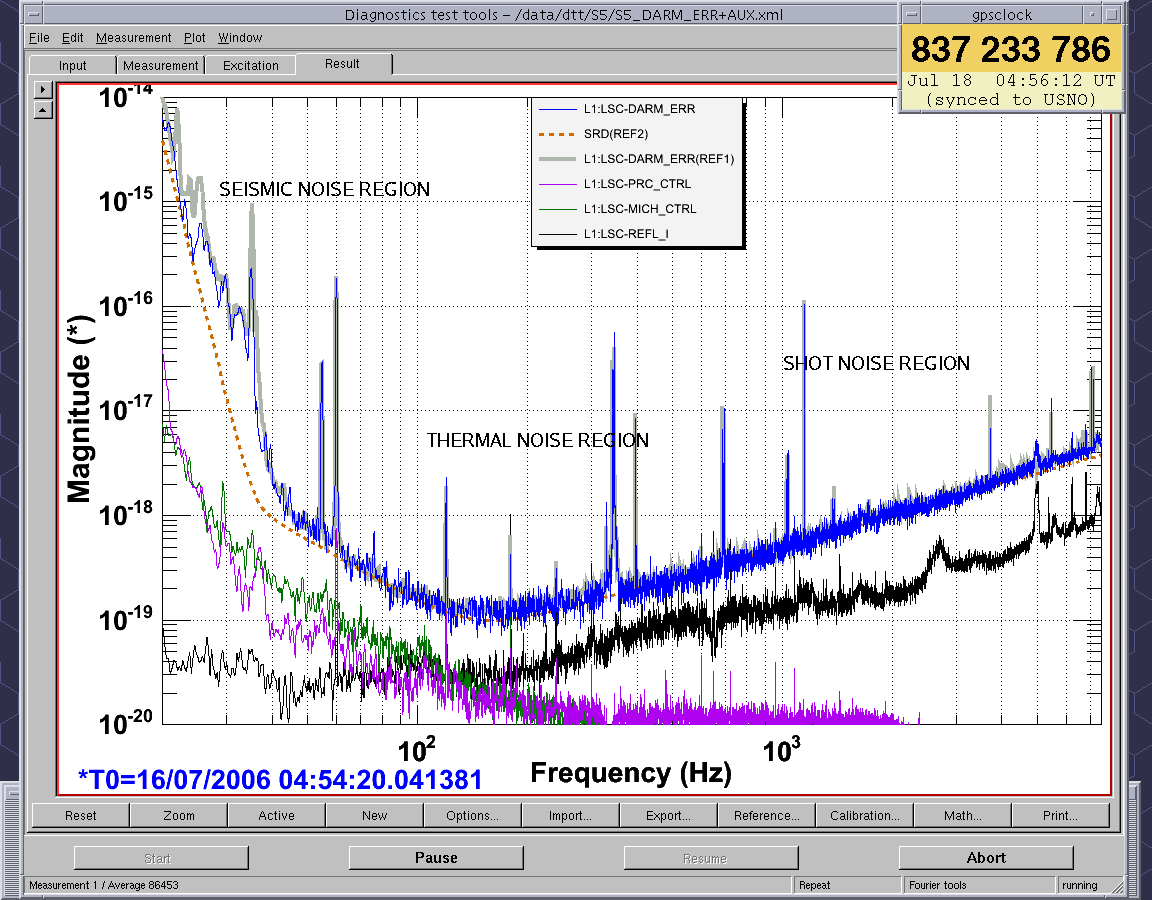
\includegraphics[width=0.7\textwidth]{chapter2/spectrum.png}
%\caption{\label{f:spectrum}LLO noise spectrum}
%\end{center}
%\end{figure} 
%\SECTION{TBD}
%\SUBSECTION{TBD}

\chapter{DC Readout}
\label{chapter3}

The initial LIGO detectors used RF heterodyne detection, inspired by
the Pound-Drever-Hall technique, to sense all interferometer length
degrees of freedom and most angular degrees of freedom.  During
Enhanced LIGO, the sensing of the gravitational wave channel (DARM)
was changed to a form of homodyne detection called DC readout.  In
this chapter I explain the motivation for and theory behind DC
readout.

\section{Principle of DC readout}
A homodyne readout system differs from a heterodyne system by using a
local oscillator at the same (optical) frequency as the field we wish
to measure.  In DC readout we bring this 

DC readout creates a homodyne local oscillator by putting a small
offset into the Michelson or DARM degree of freedom, moving the
interferometer slightly off of the DARM fringe at DC.  In this
``fringe'' view, the operation is very simple to understand: moving
off of the null point introduces a non-zero first derivative.  

The true beauty of this technique is that it exploits the filtering
action of the compound interferometer to produce the local oscillator;
any fluctuations in the amplitude or frequency of the input laser
field are attenuated by the coupled cavity pole before reaching the
output port.

\section{Motivation for DC readout}

Some of the motivations of DC readout and an output mode cleaner are:

\begin{itemize}
\item The filtering action of the compound interferometer produces an
  extremely quiet local oscillator.  This reduces the coupling of
  laser noises to the readout.
\item Contributions from noise on the electronic oscillator used to
  create the RF sidebands are greatly reduced.
\item The shot-noise-limited sensitivity of homodyne detection is
  inherently better than that of heterodyne detection, for a fixed
  amount of power on the detection photodiodes, by a factor of at
  least $\sqrt{3/2}$.
\item The shot noise level may be further reduced through the
  injection of squeezed quantum vacuum.  This is much more technically
  feasible with homodyne detection than heterodyne detection.  This
  has recently been demonstrated at the GEO600 detector and a
  prototype implementation is underway at Hanford.
\item In DC readout, the signal field and the local oscillator are
  guaranteed to have perfect spatial overlap, since they come from the
  same place.  By contrast, in the conventional heterodyne
  arrangement, the RF fields and the carrier are resonant in different
  cavities and may occupy slightly different spatial modes.  This
  leads to a reduction of shot-noise-limited SNR.  (However, an output
  mode cleaner can be used to force good overlap in either case.)
\item The output mode cleaner greatly decreases the amount of power
  that must be detected by the detection photodiodes by removing
  spurious higher order modes.    
\end{itemize}

\begin{figure}[p]
\includegraphics{figures/fields-picture.pdf}
\caption[Frequency-domain fields in DC and RF
  readouts]{\label{fig:sideband-picture}Depiction of the fields in DC
  and RF readouts.  (a) In RF readout, the laser carrier is suppressed
  by operating the Michelson on a dark fringe for the carrier.
  Differential phase modulation in the arms becomes amplitude
  modulation of the (suppressed) carrier, depicted as the
  audio-frequency sidebands at $\pm f_{gw}$.  The photodiode sees a
  beat between the GW signal and the RF sidebands.  In homodyne
  readout, a carrier-frequency local oscillator is introduced--in DC
  readout this is done by introducing a microscopic asymmetry between
  the two arms.  The RF sidebands are no longer needed and are removed
  by the output mode cleaner.  The GW-induced sidebands appear as
  amplitude modulation on the carrier, which is sensed directly by the
  photodiodes.}
\end{figure}

\begin{figure}[p]
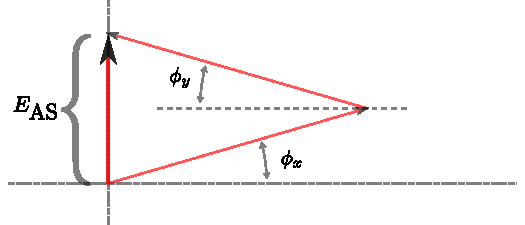
\includegraphics[width=\columnwidth]{figures/phasors.pdf}
\caption[Phasor diagram of DC readout]{\label{fig:mich-phasors}Phasor
  diagram of the fields at the AS port due to the two arms of the
  Michelson.  DARM motion causes equal but opposite rotation of the
  two phasors, which modulates the amplitude of the resultant electric
  field at the AS port ($E_{AS}$).  If this field has a nonzero
  nominal value, as in DC readout, then this will also result in
  linear modulation of $P_{AS}$.}
\end{figure}

\subsection{Calculation of the optical gain}

The ratio of signal produced (in Watts) to displacement of DARM (in
meters) is the \emph{optical gain}.  In DC readout, we can find the
optical gain for slow DARM variations by simply taking the derivative
of the power at the anti-symmetric port with respect to changes in
DARM.

From the prior chapter, take the expression for the power at the
output of a Michelson:
\begin{equation}
P_{AS} = \frac{1}{4}P_{BS}\left( {r_+}^2 \sin^2 \phi_- + {r_-}^2 \cos^2 \phi_-\right)
\end{equation}
Neglecting the difference in reflectivity, we have simply
\begin{equation}
P_{AS} = P_{BS} \sin^2 137 k x
\end{equation}
where $k=2\pi/\lambda$ is the wavenumber, $x$ is the DARM displacement, and $137$ is the phase gain.
Taking the derivative, we find the optical gain
\begin{align}
S_{DC}  & = \frac{\partial P_{AS}}{\partial x}  \\
       & = 2 P_{BS} \sin (137 k x) \cos(137 k x) 137 k \\
       & = 2\cdot 137 k \sqrt{P_{BS} P_{AS}} \cos(137 k x)
\end{align}
The cosine term is very near unity and can be neglected.  Also, the
phase gain dies off with the cavity pole; and $P_{BS}$ is related to
the input power $P_{IN}$ via the power recycling gain ${g_{cr}}^2$.
Putting this together, we get:
\begin{equation}
S_{DC}(f) = 2 g_{cr} \sqrt{P_{IN} P_{AS}} \left(\frac{r_c'}{r_c}\right) \left(1 + i\frac{f}{f_c}\right)^{-1}
\end{equation}

%% To the extent that the introduction of DC offset simply creates a
%% nonzero carrier field at the output port and does not otherwise affect
%% the interferometer dynamics, the frequency response of the interferometer
%% is the same in DC readout as in heterodyne readout, except for an
%% overall scaling. This can be seen by considering the sideband picture
%% (see Figure \ref{fig:sideband-picture}) and is borne out by the following
%% derivation.%

We see that the optical gain scales with the square root of both input
power and the power at the AS port (assuming that the power recycling
gain $g_{cr}$ remains constant, which is approximately true for small
offsets).  From this we can conclude several properties of DC readout
immediately:
%
\begin{itemize}
\item Because the optical gain and the shot noise ASD both scale with
  $P_{AS}$, the shot-noise-limited sensitivity is insensitive to the
  particular DARM offset we use.
\item The sensitivity of the detector improves with the square root of
  the input power.
\item The frequency response of the interferometer is the same in DC
  readout as in RF readout, up to a scaling factor. (Both are shaped
  simply by the cavity pole.)
\end{itemize}
%
As long as the DARM offset is sufficiently small, the degradation of
power recycling is negligible.

\begin{figure}[p]
\centerline{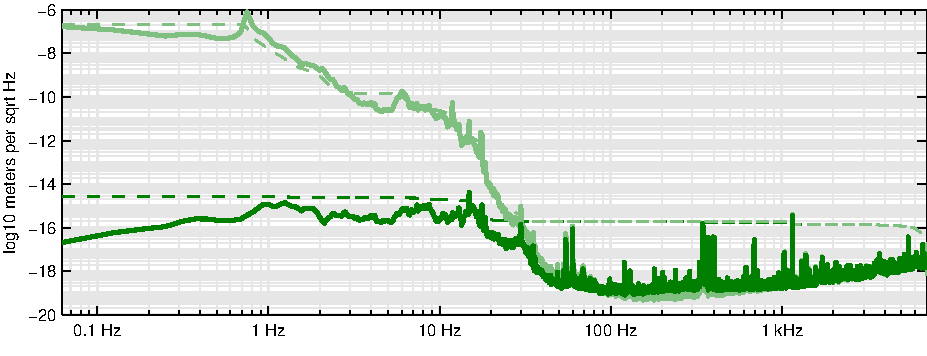
\includegraphics[width=\columnwidth]{figures/residualDARM.pdf}}
\caption[Residual DARM motion]{\label{fig:residual-DARM}DARM
  motion. The lower trace shows the residual motion of DARM after
  stabilization by the DARM control loop.  The upper trace shows the
  `calibrated' DARM, in which the effect of the control loop has been
  removed by multiplying by $(1+G)$, where $G$ is the open loop gain;
  this can be interpreted as `the motion that would be there if there
  were no control loop.'  The control loop reduces the RMS DARM motion
  by ten orders of magnitude in order to hold the interferometer
  within the linear regime around the operating point.  The DARM
  offset used to implement DC readout must be significantly larger
  than the RMS residual motion ($\sim10^{-14}$ m) to avoid fringe
  wrapping and nonlinearity.}
\end{figure}

\subsection{Decrease in arm power due to off-resonance operation}

The decrease in buildup for a cavity operated off-resonance goes like
$(2\mathcal{F}/\pi)^2\phi^2$, where $\phi$ is the cavity detuning.
For $\mathcal{F}=220$ and $\phi=(2\pi/1064\text{ nm})(10\text{ pm})$,
the fractional power loss is only $7\times10^{-5}$.

\subsection{Decrease in power recycling gain due to power loss at the output port}

Allowing power to escape the power recycling cavity (PRC) through the
AS port effectively increases the losses of the PRC, diminishing the
power recycling gain.

The carrier power in the PRC is given by
\begin{equation}
P_{BS} = P_{IN}\left| \frac{t_{RM}}{1 - r_{RM} r_{IFO}}\right|^2
\end{equation}
where $t_{RM}$ is the amplitude transmissivity of the recycling
mirror, $r_{RM}$ is its reflectivity, and $r_{IFO}$ is the amplitude
reflectivity of the rest of the Fabry-Perot Michelson interferometer.
The power-recycling cavity is designed to be critically coupled, so
$r_{IFO}\approx r_{RM}$.

With a DC offset in place, the reflectivity of the Michelson becomes $r_M = r_{IFO}\cos\phi_-$, so we can write
\begin{equation}
P_{BS}(\delta x) \approx P_{IN} 
\frac{T_{RM}}{\left(1 - R_{RM} \cos\left(2\cdot137\cdot k\cdot\delta x\right)\right)^2}
\end{equation}
The loss of power recycling gain becomes significant for large
offsets.  For a 10 pm offset, the reduction in power recycling gain is
only 1\%, but for a 50 pm offset it grows to 20\%.

\subsection{DC readout elsewhere}
DC readout has been implemented previously at the Caltech 40 meter
prototype \cite{Ward2008DC,RobWardThesis} and the GEO 600
detector\cite{GeoDC,Prijatelj2010,Degallaix2010Commissioning}.  The
current configuration of Virgo incorporates an output mode cleaner but
uses RF heterodyne readout\cite{Acernese2008Virgo}.

\begin{figure}
\includegraphics[width=\columnwidth]{figures/dc-readout-diagram.pdf}
\caption[Enhanced LIGO interferometer
  layout]{\label{fig:dc-readout-ifo}Enhanced LIGO interferometer
  layout (not to scale).  The dotted line represents the vacuum
  enclosure. The initial LIGO configuration is modified by adding an
  output mode cleaner and DC photodiodes.  A beamsplitter directs 97\%
  of the optical power to this new path and the remaining 3\% to the
  old RF heterodyne output chain, used for lock acquisition and
  automatic alignment.}
\end{figure}

\CHAPTER{Output Mode Cleaner}
\label{chapter4}
\section{Introduction}

The optical fields in the interferometer are intended to exist in only
the fundamental Gaussian spatial mode.  A critically coupled resonant
cavity, the input mode cleaner, is used to attenuate any higher order
spatial modes produced by the laser before the field is incident on
the interferometer.  Despite having an essentially pure input beam,
imperfections in the interferometer optics leads to the production of
higher order spatial modes in the interferometer; this effect is
particularly egregious for the RF sidebands in the power recycling
cavity\cite{Gretarsson2007Effects}.  As a result, the output beam
(depicted in figure~\ref{fig:as-spot}) is no longer in the pure
Gaussian mode, but also contains spurious higher order modes.

The spurious higher order spatial modes in the output beam are
detrimental to interferometer performance as they generally produce no
useful signal, but contribute additional photon shot noise, increase
the power that needs to be detected, and exacerbate noise couplings.
To mitigate these effects, an \emph{output mode cleaner} (OMC) was
installed at the output port.  This critically-coupled optical filter
cavity attenuates higher order spatial modes before the beam is
detected by a pair of photodiodes.  In DC readout, the OMC is also
used to remove the RF sidebands, which are still needed in the
interferometer to sense other degrees of freedom, but would only be
detrimental to the DC readout signal.

\begin{figure}[t]
\centerline{\includegraphics[width=0.5\columnwidth]{figures/as_spot.png}}
\caption[Beam spot at the interferometer output port]{
\label{fig:as-spot}Image of the beam spot at the L1 output
  port taken using a CCD camera.  This image is saturated in the
  central portion but emphasizes the spurious higher order modes
  surrounding the fundamental Gaussian, including contributions
  from both the carrier and the 25 MHz sidebands.}
\end{figure}

\section{Physical Design of the Cavity}

\begin{figure}[t]
  \subfloat[][Schematic of OMC bench]{
  \includegraphics[width=0.5\columnwidth]{figures/omc-diagram.pdf}
  \label{fig:omc-diagram}
}
\subfloat[][\label{fig:OMC-chamber}Photograph of installed OMC and suspension]{
  \includegraphics[width=0.5\columnwidth]{figures/chamber-picture-smaller.pdf}
}
\caption[OMC diagram and photograph of installation]{
  (a) Diagram illustrating the design of the monolithic OMC
  bench; (b) Photograph of the installed output mode cleaner,
  suspension, and seismic isolation platform. The OMC is located in a
  dedicated vacuum chamber, separated from the main vacuum enclosure
  by a septum window, allowing rapid venting cycles during
  commissioning.}
\end{figure}
\begin{figure}
\includegraphics[width=\columnwidth]{figures/D0901817.pdf}
\caption[Output Mode Cleaner photograph]{Photograph of the Output Mode
  Cleaner used at Livingston (\emph{ex situ}).  Only one of the two DC
  photodiodes is installed in this photo.  Photometry by Sam Waldman;
  this diagram has document number
  \href{https://dcc.ligo.org/cgi-bin/private/DocDB/ShowDocument?docid=4713}{D0901817}.
}
\end{figure}
% Hanford: 
% https://dcc.ligo.org/cgi-bin/private/DocDB/ShowDocument?docid=4714


A four-mirror bow-tie arrangement was chosen for the mode cleaner
design\footnote{The Enhanced LIGO OMC design and construction was lead by
  Sam Waldman as part of LIGO's Interferometer Sensing and Control (ISC)
  group.}.  This non-colinear design prevents direct reflection of
rejected light back into the interferometer.  A design with an even
number of mirrors was preferred so that odd-parity transverse modes
are degenerate, reducing the density of higher-order-mode resonances.
A sufficiently high angle of incidence of the beam on the mirrors is
necessary to minimize the effects of small-angle scattering, subject
to the constraint that too great an angle of incidence will introduce
excessive astigmatism to the beam.

The cavity was constructed by rigidly mounting the cavity optics and
photodetectors to a baseplate, similar to the LISA optical bench
design.  The baseplate is a slab of Corning ULE glass $450 \mathrm{mm}
\times 150 \mathrm{mm} \times \mathrm{39}\mathrm{mm}$; components were
bonded using Optocast {\sffamily 3553LV-UTF-HM} UV-cure epoxy.

Two of the cavity mirrors are outfitted with position actuators: a
fast, short-range ($\lesssim0.1$ \micron) PZT, and a slow, long-range
($\approx 20$\micron) thermal actuator consisting of a 1 inch long segment
of aluminum tube warmed by a resistive heater.

%% Cavity properties [Table]
% These values are all from Sam's document T080144:
% https://dcc.ligo.org/cgi-bin/private/DocDB/ShowDocument?docid=5416
\begin{table}
\centering
\begin{tabular}{l l l l l}
\hline 
parameter          & design      & H1          & L1            & units   \\                    
\hline
perimeter ($p$)    & 1.042       & 1.077       & 1.016         & m       \\
beam waist ($w$)   & 477         & 496         & 463           & \micron \\
Finesse (\Finesse) & 400         & 360         & 360           &         \\
FSR                & 287.7       & 278.3       & 295.2         & MHz     \\  % fsr = c/p
cavity pole        & 360         & 390         & 410           & kHz     \\  % f_c = fsr/(2F)
g-factor           & 0.739       & 0.725       & 0.722         &         \\
HOM freq shift     & 69.4        & 67.2        & 71.8          & MHz     \\
transmission       & 1           & $\geq$0.95  & $\geq$0.90    &         \\
\hline
\end{tabular}
\caption[Output mode cleaner properties (designed and measured)]{Designed and measured properties of the Hanford and Livingston output mode cleaners.}
\label{tab:OMCproperties}
\end{table}

%% OMC Suspension
To isolate the mode cleaner from environmental disturbances, the
optical bench was hung from an actively-damped double-pendulum
suspension system\cite{Robertson2006Conceptual,Robertson2009OMC},
which was in turn suspended by an in-vacuum active isolation
system\cite[Chapter 5]{KisselThesis}.

%% OMC Photodiodes
The photodiodes were also mounted on the OMC baseplate, and read out
by in-vacuum preamplifiers.  The output from the mode cleaner was
split via a 50/50 beamsplitter and directed to two Perkin Elmer 3mm
diameter InGaAs photodiodes (part number C30665GH), with measured
quantum efficiency $> 0.95$ at 1064 nm.  The photocurrent was
converted to voltage across $100 \Omega$ transimpedance. Subtraction
of the signals from the two photodiodes produces a diagnostic
``nullstream'' containing the anti-correlated component of the PD
signals.
%
The rigid mounting of the PDs to the OMC baseplate reduces the
possibility of beam motion coupling to photocurrent through photodiode
nonuniformities, and the in-vacuum preamplifiers reduce the liklihood of
electronic or triboelectric noises.

\section{Requirements}

The OMC is required to sufficiently filter the light present at the
output port such that contributions from the RF sidebands and higher-order
spatial modes become negligible. To exclude the RF sidebands, the
cavity length is chosen such that the RF sideband frequencies are
anti-resonant in the cavity, which yields minimum transmission.

\section{Choosing the OMC Finesse}

All else being equal, we want the best possible filtering capability
from the OMC.

The transmission of a lossless critically-coupled cavity is given by
\begin{equation}
T = \frac{1}{1 + \frac{4}{\pi^2}\mathcal{F}^2\sin^2\phi}
\end{equation}
where $\mathcal{F}$ is the cavity finesse and $\phi$ is the cavity's
detuning from resonance.  Since the cavity will be locked to resonance
for the laser carrier, to find the attenuation of other modes, we set
$\phi$ to the detuning of these modes.

The maximum attenuation of a mode is given by $(4/\pi^2)\mathcal{F}^2$.

After filtering by the OMC, we want the shot noise contributions from
unneeded modes to be negligible, and the contribution from noises on
these fields to also be negligible.  Almost any cavity would be
sufficient to reduce excess shot noise contributions.  The need for a
high finesse OMC comes from the need to eliminate audio frequency
noises carried on the RF sidebands and higher-order spatial modes.

\begin{comment}
 h = 6.626068e-34;
 c = 299792458;
 lambda = 1064e-9;
 nu = c / lambda;
 P = 100e-3;
 shotnoise_RIN = sqrt(2*h*nu/P)
\end{comment}

Consider the contribution of intensity noise on the RF sidebands.  Any
residual intensity noise on the RF sidebands will contribute directly
to the DC readout signal.  Assume that the carrier has about 100 mW
power and that the RF sidebands have about the same amount of power,
and assume that the laser intensity noise is $10^{-7}$ RIN.  The shot
noise RIN on 100 mW is (per equation~\ref{eq:shotnoise-asd})
$\sqrt{2h\nu/P} \approx 2\times10^{-9}$.  Thus we need to attenuate
the RF sidebands by at least a factor of 100.

The RF sidebands will not be exactly anti-resonant in the cavity but
will actually lie at about $0.1 fsr$ away from the carrier.  Thus the
attenuation is diminished by approximately $\sin^{-2} (0.1 \pi)
\approx 10$.  So we need attenuation of 1000.  But we really want at
least a factor of 10 margin, so we'll want maximum attenuation of
10000. This means we need a finesse of at least 160.

On the other hand, higher finesses lead to greater net power loss as
the beam travels through the cavity, as the intra-cavity loss is
multiplied by each effective roundtrip in the cavity.  To choose the
finesse, we assume a roundtrip intra-cavity power loss of 100pm and
set the constraint that the net power efficiency of the OMC should
exceed 99\% (not actually achieved).  This leads to the design choice
of a finesse of 400.

\section{Choosing the OMC Length and Geometry}

The cavity length is chosen to provide adequate attenuation of the RF
sidebands, and its geometry ($g$-factor) is chosen to sufficiently
attenuate higher-order modes.  The optimal g-factor depends on the
specific details of the frequency and spatial spectrum of modes at the
output port.  These depend strongly on the details of the
interferometer optics, alignment, and thermal state. 

To deal with these unknown factors, we designed the OMC using a model
in which the power in each higher order mode (of order $n$) was proportional to
$1/n^2$ and the RF sidebands had their nominal power.  The designed
and as-built properties of the output mode cleaner cavities are given
in Table~\ref{tab:OMCproperties}.
%
One disadvantage of the chosen design is that the 4-th order mode is
nearly degenerate with the fundamental mode.  We did experience
problems with accidental degeneracy in one of the mode cleaners, which
was addressed by changing the operating temperature of the thermal
actuator (which had a small coupling to the effective radius of
curvature of the mirror).  The next version of the output mode cleaner
will be designed with a slightly different g-factor to avoid this
problem.


\section{OMC Feedback Control Systems}

%% Front-end Computers 
The mode cleaner was controlled and the DC readout signals were
acquired using a prototype of the advanced LIGO real-time digital
signal processing system, consisting of a Linux-based computer
equipped with analog-to-digital and digital-to-analog converters and
interfaced to other systems via reflected memory over a fiber ring and
EPICS over ethernet, operating at 32768 samples per second (Hz) The
LIGO Realtime Code Generator\cite{Bork2009ELIGO,Bork2009AdvLigo}
allowed fast prototyping and implementation of complex servos.  All
servos involving the OMC were implemented using this digital system.

\subsection{Length Sensing and Control (LSC)}

The cavity length must be controlled to maintain the resonance of the
laser carrier.  To sense the mismatch between the laser carrier and
the cavity length, we modulate the cavity length by a small
displacement at high (audio) frequency and monitor the transmitted light
intensity for a signal at the same frequency.  Cavity transmission is
a quadratic function of the frequency/length mismatch; if the
modulation is perfectly symmetric around the point of peak
transmission, there will be no linear coupling.  Effectively, we sense
the first derivative of the transmission with respect to cavity
length.  

\begin{figure}[t]
\centerline{\includegraphics[width=0.5\columnwidth]{figures/ditherdoodle.pdf}}
\caption[Cartoon view of dither locking]{\label{fig:dither-doodle}Cartoon view of dither locking.  The dither locking technique allows a system to be locked to a quadratic operating point.  For example, dither locking is used to control the OMC cavity length, where, near resonance, transmission is a quadratic function of cavity displacements.  A sinusoidal modulation is injected into the parameter we wish to tune (i.e. cavity length), and the output (i.e. transmitted light intensity) is demodulated at the same frequency, producing an error signal.  The figure shows the phase-flip that occurs as the system moves through the quadratic point.  At the quadratic point, the error signal is zero, while on either side it attains nonzero values with opposite signs.}
\end{figure}

\subsubsection{Modeling the Dither Locking}

Suppose $f(x)$ is a function we wish to maximize; in this case, $f$
gives the power transmitted through the OMC as a function of length
offset.  We let $x = x_0 + A \cos\omega t$, where $A$ is the amplitude
of the dither and $\omega$ is its frequency.  We can expand $f$ as a
power series around $x_0$: 
\begin{align}
f(x) &\approx f(x_0) + f'(x_0)\left(x - x_0\right) + f''(x_0)\left(x-x_0\right)^2 + \cdots \\
     &\approx f(x_0) + f'(x_0)A\cos\omega t        + f''(x_0)A\cos^2\omega t + \cdots
\end{align}
%
The amplitude of the $\cos\omega t$ term is proportional to the first
derivative of $f$ at the current operating point.  (There are also
contributions from higher derivatives, but we assume the lower
derivatives dominate.)

\subsubsection{Noise limits}

Suppose the OMC has coefficient of finesse $F$ and $P$ watts on the
photodiode.  The dither amplitude is $A$ and dither frequency is
$\omega$.  What is the sensing noise limit?

The background is Gaussian white shot noise, equally distributed into
the two demodulation quadratures.  So the noise floor of the
demodulated signal is $(1/\sqrt{2})\sqrt{2 h \nu P}$.

The transmission of the OMC goes like $T(x) = 1/\left(1 + Fx^2\right)$
which has first derivative $T'(x) = 2 F x / \left(1 + F x^2\right)^2 =
- 2 F x + O(x^2)$.  Thus the optical gain is $-2 F A$ watts per meter.

The fast PZT actuator is dithered at 10 kHz and this signal is
synchronously demodulated in the transmitted light.  The bandwidth of
the servo is about 100 Hz.

\section{Input Beam Alignment Sensing and Control (ASC)}

In addition to controlling the cavity length to keep the carrier
resonant, we must control the pointing of the beam incident on the
OMC.
Aligning the input beam to the OMC is a significant problem, since the OMC
can only clean the light insofar as we can identify the mode we want to
keep.

The decomposition of a given optical field into Hermite-Gauss
eigenmodes is dependent upon a choice of origin and spot size.  The
OMC cavity will select the projection of the incident field onto its
eigenmode.  The optics directing the interferometer output beam to the
OMC

Several OMC alignment schemes were implemented and utilized.

\subsection{QPD Alignment}

The simplest alignment control simply uses the two quadrant
photodiodes (QPDs) mounted on the OMC breadboard.
These are simply photodiodes whose surfaces are divided into
four quadrants.  By subtracting the power seen on one half
of the QPD face from the power seen on the other half, we 
can measure the position of the incident beam.

Alignment servos based on the QPDs have the advantage of being very
robust and not requiring that the OMC already be locked, and so are
ideal for initial alignment of the OMC before locking the cavity.  The
QPD alignment, however, has no notion of the ideal DC pointing of the
beam and is sensitive not just to the carrier, but also the RF
sidebands.

\subsection{Dither Alignment}

A second alignment scheme is to dither the two steering mirrors each
in pitch and yaw, demodulate the OMC transmitted signal at these
frequencies, and feed back to the mirrors--exactly analogous to the
operation of the OMC length control system. 

The basic dither alignment scheme has some attractive features, but
does not work properly in the presence of spurious higher order
modes--the exact problem which motivates the use of the OMC in the 
first place.

Dither alignment works maximizes the power transmitted through the
OMC; because this is a quadratic maximum of transmission versus
pointing, the linear coupling of beam jitter to the transmitted
intensity is nulled.  However, this technique cannot distinguish
between the optical field coming from the interferometer arms, and any
higher order modes of the carrier resonant in the PRC.  If there is
carrier power in the TEM01 mode, this servo will misalign the input
beam slightly, to convert the incident TEM01 mode into the TEM00 mode
of the cavity.  (The conversion of TEM01 to TEM00 via beam displacement
is depicted in figure~\ref{fig:dithermax}.)

\begin{figure}
\includegraphics{figures/dithermax.pdf}
\caption[Modal decomposition of a displaced Gaussian]{\label{fig:dithermax}The sum of a gaussian and a first-order higher order mode
  resembles a displaced gaussian.  A basic dither alignment scheme,
  which maximizes the power transmitted through the OMC, would
  operate near point B, rather than point A.}
\end{figure}

%% RF Wavefront sensing.  We did not really consider this.

%% AF IM WFS.  The same OMC length dither which is used to lock the cavity
%% length produces an audio-frequency sidebands of the OMC mode in
%% reflection.  The beats between this light and the light rejected from
%% the OMC on a pair of photodiodes can be used to produce alignment
%% error signals.

%% Beacon dither.  

%% SNR dither.  Nicolas's scheme.
\subsection{Drumhead Dither OMC Alignment System}

\begin{figure}
\includegraphics{figures/drumhead-dither.pdf}
\caption[Drumhead dither system]{The `Drumhead dither' OMC alignment
  system.\label{fig:drumhead-dither}}
\end{figure}

From the experience with basic dither alignment, it is clear that what is
needed is some alignment system which can specifically detect the arm
cavity mode.  To accomplish this, we `tag' the light in the arm cavity by
modulating the arm length at high frequency and looking for this modulation
in the light transmitted through the OMC. 

The system was implemented as follows:

\begin{enumerate}
\item One of the arm cavity lengths is modulated at high frequency, 9
  kHz.  Intuitively, this modulation `tags' the carrier light emerging
  from the arm.  The modulation is accomplished with a small drive by
  feeding the mechanical drumhead mode of the test mass. (This gives
  rise to the nickname of the method, `drumhead dither'.)
\item The spectral power of the 9 kHz line in the OMC photodiode
  signal is measured by bandpassing the signal around 9 kHz, squaring
  the result, and then low pass filtering.
\item The four degrees of freedom of the two beam steering mirrors are
  modulated (dithered) at a frequency slow compared to the low pass
  filtering in step (2).
\item The measured power in the 9 kHz line is demodulated at the
  steering mirror dither frequencies, producing alignment error
  signals which are fed back to the mirrors.
\end{enumerate}

This system is depicted in figure~\ref{fig:drumhead-dither}.

%\subsection{Optimal OMC Alignment}

It has been pointed out~\cite{Smith2011Optimal} that even the drumhead
dither alignment scheme is not optimal in the sense of producing the
best shot-noise-limited SNR.

\begin{comment}
\section{Automatic Gain Control (UGF servo)}
% FIXME - Gaby says: This is very obscure - if you don't have time to
% explain more, just skip it...
The optical gain of the interferometer naturally varies slowly as
alignment drifts and the thermal state of the mirrors changes.  The
over-all loop gain must be kept within a few dB of its nominal value
in order for the loop to remain stable.

Before S6 this was done by periodically running a script which
measured the loop gain and adjusted a digital gain to bring it to
nominal.

The flexibility of the realtime code generator allowed us to implement
an automatic gain control servo directly in the OMC front-end.  This
was a nice convenience. 
\end{comment}

%% \subsection{Mode scan}

%% With the interferometer controlled using the heterodyne readout, the
%% Output Mode Cleaner can be used as a mode analyzer cavity by varying
%% the cavity length by at least a free-spectral-range. Because this
%% range is more than the fast PZT actuator, this is accomplished by
%% putting a large step into the thermal actuator.
%%  These mode scans can
%% address questions such as:
%% \begin{itemize}
%% \item How well aligned is the OMC?
%% \item How well mode-matched is the OMC?
%% \item How much carrier power is at the output port compared to sideband
%% power?
%% \item How well balanced are the RF sidebands?
%% \item How much junk light is present at the output port?
%% \item Are there any nasty modes near the 00 mode that will sneak through?
%% \item The horizontal/vertical mode separation
%% \end{itemize}
%% The mode scan cannot, by itself, distinguish carrier mode light from
%% the arms vs carrier mode junk light.


\section{Scattering}

Viewed from the output port, the interferometer appears almost
perfectly reflective.  Any light scattered (i.e. retroreflected) by
the output optics at a small angle could scatter into the
interferometer mode, reflect off of the interferometer, joining (and
interfering with) the main interferometer signal and LO beam.  Any
modulation of the path length between the main interferometer and the
backscatterer will change the interference condition, producing
intensity variations in the OMC transmitted beam and contaminating the
DARM readout.

\subsubsection{Measuring the OMC Scattering Reflectivity}

The backscattering reflectivity of the OMC can be experimentally
measured by intentionally modulating the path length between the
interferometer and the OMC.  This produces phase modulation in the
backscattered field.  This phase-modulated field reflects from the
interferometer and combines with the local oscillator field.   

\begin{figure}[t]
\includegraphics[width=\columnwidth]{figures/scat_fd.pdf}
\caption[Measurement of OMC
  backscatter]{\label{fig:scattering}Measurement of effective OMC
  backscattering reflectivity.  With the interferometer operating in
  low-noise mode, we excited (modulated) the position of the OMC in
  the direction of the incident beam, thus modulating the path length
  between the interferometer and the OMC.  This produces the
  characteristic `scattering shelf' spectrum in the power at the OMC
  photodiodes.  Integrating the area under the shelf and dividing by
  the DC power gives the effective backscattering reflectivity. (The
  photocurrent has been corrected for the suppression of the DARM
  control loop.)}
\end{figure}

The backscattered beam has an electric field amplitude of
%
\begin{equation}
E_s = a E_0 \exp\left\{ i \frac{2 A}{\lambda} (2 \pi) \sin \Omega t \right\}
\end{equation}
%
where $A$ is the amplitude (in meters) of motion of the scatterer,
$\Omega$ is the frequency of motion, and $a$ is the amplitude
reflectivity of the scattering source (the scattering
coefficient). This is phase modulation with a modulation depth of
%
$\Gamma = 4 \pi (A/\lambda)$
%
radians, assuming normal incidence on the scatterer.  The photodiode
detects the power in the resulting field, which is
%
\begin{align}
P &= |E_t + E_s|^2 \\
  &= |E_t|^2 + |E_s|^2 + 2 \text{ Re } E_t E_s \\
  &= |E_0|^2 + 2 \text{ Re } E_t E_s
\end{align}
where $E_t = (1 - a) E_0$ is the field that's transmitted rather than
scattered.
%
Using the Jacobi-Anger identity, $E_s$ can be expanded in terms of
sinusoids to find the power spectrum of the photodiode signal:
%
\begin{align}
P &= |E_0|^2 + 2 \text{ Re } E_s {E_t}^* \sum_{n=-\infty}^{\infty} i^n J_n(\Gamma) \exp{i n \Omega t} \\
  &= |E_0|^2 + 2 |E_0|^2 a (1 - a) \text{ Re } \sum i^n J_n(\Gamma) \exp{i n \Omega t} 
\end{align}
%
We are interested not only in the case of small modulation depth
(i.e. small motion of the scatterer), but also very large modulation
depths, greater than the wavelength of the light, which produces many
higher order harmonics.  Spectrally, this looks like a comb of delta
functions at integer multiples of $\Omega$, whose amplitudes are given
by bessel functions $J_N(\Gamma)$ with $N=f/\Omega$.  Any noise on the
carrier will get superimposed on each of these spikes, smoothing out
the observed spectrum.

Large motion of a backscatterer produces a characteristic `shelf'
feature in the PD spectrum (c.f. figure~\ref{fig:scattering}).  This
is because the amplitude of Bessel functions $J_N(\Gamma)$ dies off
very steeply with $N$ after $N>\Gamma$, creating the characteristic
`scattering shelf'.  The cutoff (`knee') frequency therefore occurs
when $N \approx \Gamma$; the knee frequency may be calculated as
follows:
%
\begin{align}
f_{knee} & = \Omega N_{knee} \\
       & = \Omega \Gamma \\
       & = 4 \pi \Omega (A / \lambda)
\end{align}

Another way of seeing this is to consider the (time dependent) phase
induced by the scatterer and take its derivative to find the maximum
frequency shift due of the backscattered light:
%
\begin{align}\
\phi &= \Gamma \sin \Omega t\\
f_\text{instantaneous} &= d \phi/dt = \Omega \Gamma \sin \Omega t\\
\max f_\text{instantaneous} &= \Omega \Gamma
\end{align}
%
which gets the same result. An excitation of amplitude $A$
and frequency $\Omega$ has maximum velocity $v = A \Omega$. This can be
used to eliminate both $A$ and $\Omega$ from the knee frequency:
%
\begin{equation}
f_{knee} = 4 \pi (v / \lambda)
\end{equation}

Of course, we are more interested in determining the backscattering
reflectivity than details of the resulting spectrum.  There are two
principle ways to recover the scattering reflectivity: (1) Because
$\sum J_N(\Gamma)^2$ over all N equals 1, we can integrate the power
spectrum of the photodiode signal to directly measure $2 |E_0|^2 a (1
- a)$. We can then divide by the DC term ($|E_0|^2$) to get the
scattering coefficient.  (2) We can simulate the scattering process in 
the time domain, find the spectral density of the resulting signal,
and fit the model to the observed spectrum.

This procedure was carried out using the actuators in the table
supporting the OMC to produce modulations in the direction of the
incoming beam of 16 microns at 0.3 Hz and 33 microns at 0.3 Hz; the
resulting OMC transmitted spectra are shown in
figure~\ref{fig:scattering} along with a quiescent spectrum for
reference.  (The experiment was repeated with modulations in
orthogonal directions; as expected, the effect was much less than the
modulation in the beam direction.)

\begin{figure}
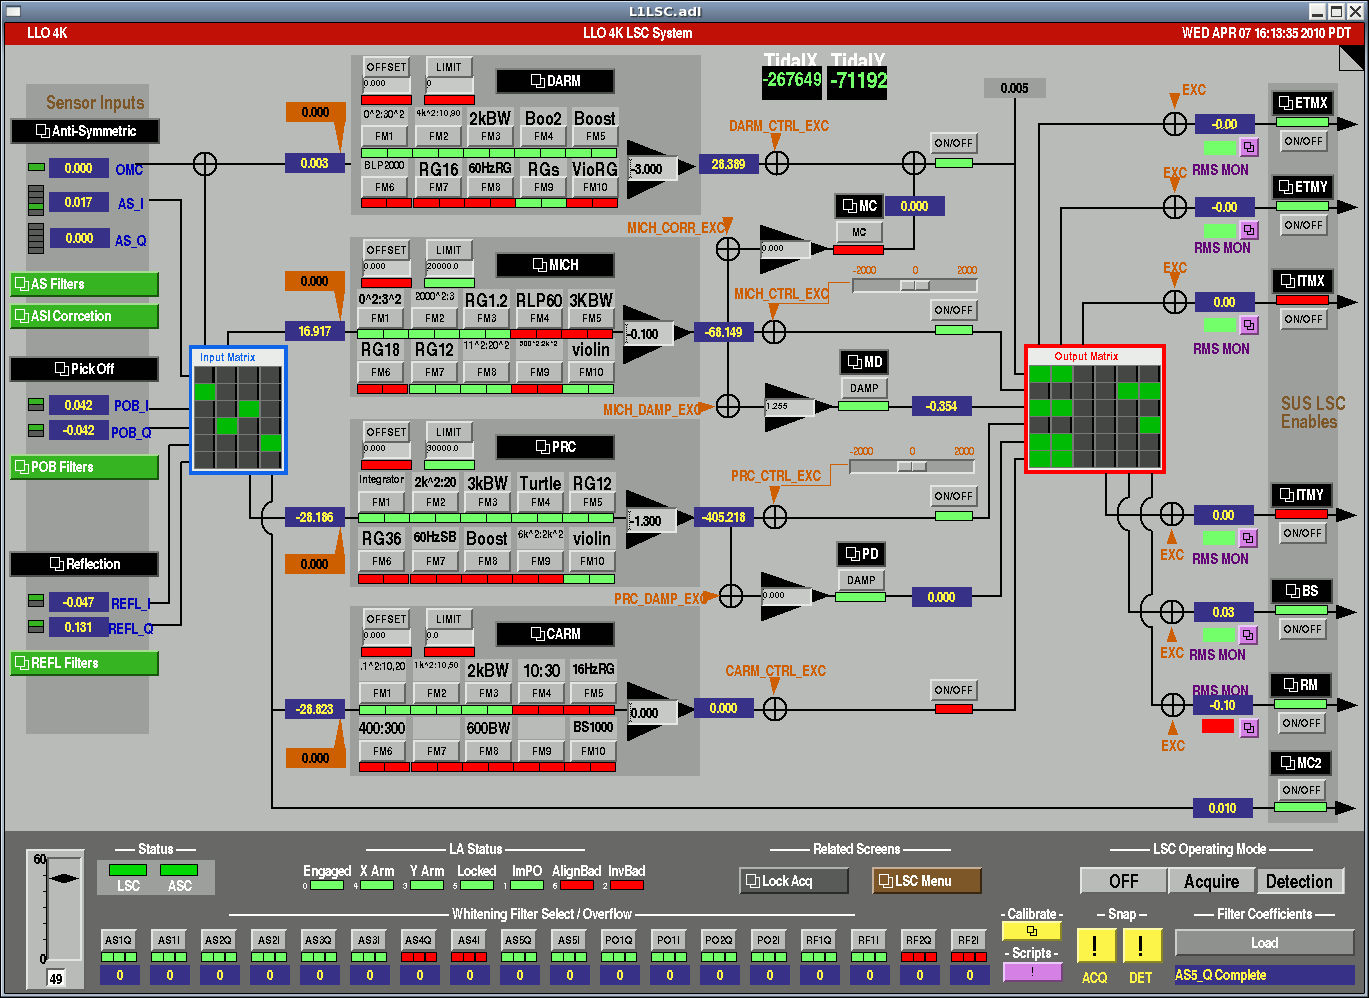
\includegraphics[width=\columnwidth]{figures/L1LSC.png}
\caption[Length Sensing and Control (LSC) control screen]{The control screen for the Length Sensing and Control
  subsystem at Livingston.  The control screen depicts signal flow in
  a generally left-to-right manner.  Photodiodes at the anti-symmetric
  (AS), pick-off (PO), and reflected (REFL) ports are indicated on the
  extreme left.  These signals are combined via an input matrix to
  form the DARM, MICH, PRC, and CARM degrees of freedom.  These
  signals are processed through an array of filter banks defining the
  control filters.  Finally, the signals pass through an output matrix
  and are then directed to the individual optics.}
\end{figure}

\section{Beam Diverter}

When the interferometer loses lock, the stored power must be dumped
somewhere. Typically, due to the presence of the power recycling mirror,
the stored power comes out the output port. This high-power transient
is sufficiently strong to burn the detection photodiodes. In order
to prevent this, one of the steering mirrors is used as a fast shutter.
It is able to zero the transmission through the OMC in approx 2 ms.

\begin{comment}
\section{Observed Beam Motion}

FIXME: Put in plots of the measured beam motion, for posterity.
\end{comment}

\section{The Front End}
\begin{comment}
% FIXME - Gaby says: This is very cute, but it may take too long to do
% a proper job... again, in the interest of time, you may just skip a
% description of the front end.

\begin{quote}
\emph{Be exhorted:} you really can predict the noise floor accurately--to
accept a noisy front end is one of the stupidest and most expensive
mistakes you can make in designing sensitive optical
instruments. Measure it, and make sure you can explain every half
decibel. -- Phil Hobbs, \emph{Building Electro-Optical Systems} \cite{Hobbs2009Building}
\end{quote}
\end{comment}

To achieve the touted SNR improvement of DC readout it is imperative
that the signal not be lost to optical losses, non-optimal photodiode
quantum efficiency, or electronics noise.

\subsection{Photodiodes}
% H1 OMC DC PDs
% https://dcc.ligo.org/DocDB/0005/T0900420/001/T0900420-v1.pdf

Sub-optimal photodiode efficiency counts as a loss just like any other
optical loss. 

The OMC photodiodes are configured in a reverse-biased,
photoconductive arrangement.  An ideal photodiode in such a
configuration will allow one charge carrier to cross the junction for
each incident photon.  The ratio of photocurrent to incident power on
the photodiode is its \emph{responsivity}.  The ratio of a
photodiode's actual responsivity to the ideal is its \emph{quantum
  efficiency}.  At 1064 nm the ideal responsivity is
%
\begin{equation}
\frac{q_e}{h \nu} = \frac{q_e \lambda}{h c} \approx 0.86 \text{ Amps/Watt}
\end{equation}
where $q_e\approx 1.6\times10^{-19}\text{ C}$ is the electron charge.

\begin{comment}
 h = 6.626068e-34;
 c = 299792458;
 lambda = 1064e-9;
 qe = 1.60217646e-19;
 responsivity = qe * lambda / (h * c)
\end{comment}

One lesson (re-)learned during Enhanced LIGO is the need to measure
the characteristics of every individual noise-sensitive component
installed in the final machine rather than relying on measurements of
test samples or typical values.  The photodiodes we originally
installed turned out to have quantum efficiency $\lesssim$ 0.60 while
the test articles of the same part number had quantum efficiency
within a few percent of unity.  Clearly there had been some change in
the manufacturing process that resulted in a greatly diminished
quantum efficiency.  Even for parts which do not show such a dramatic
systematic change, characteristics of individual parts come from some
distribution, and by measuring a batch of parts, the lowest noise
components can be hand picked.

In September 2009 we replaced the bad phototdiodes.  The replacement
photodiodes are Perkin Elmer 3mm InGaAs diodes, part number C30665GH.
The measured quantum efficiency was consistent with unity~\cite{Rollins2009H1}.

\subsection{Electronics}
An optical power of 100 mW on the readout photodiodes will produce a
photocurrent of $i = q_e\lambda/(hc)\cdot 100\text{ mW } = 86\text{ mA}$, which
in turn has a shot noise floor of $\sqrt{2 q_e i}\approx 500 \text{
  pA}/\sqrt{\text{Hz}}$.  Across $100\ \Omega$ transimpedance, this becomes $50
\text{ nV}/\sqrt{\text{Hz}}$.  The noise floor of the readout electronics must
be below this level and not be polluted by any baseband $1/f$ flicker noise.

The main strategy is to aggressively amplify the electronic signal as close to
the photodiodes as possible, so that noises added downstream become
insignificant.  To eliminate even triboelectric effects, the first preamp stages
are placed in-vacuum.  The in-vacuum preamps consist of active filter stages
with two zeros at 8 Hz and two poles at 80 Hz, for a factor of 100 amplification
at 100 Hz.  This is followed by two more pole-zero pairs in satellite amplifiers
on the floor outside the vacuum chamber, for a total gain of 10,000 before the
long run to the racks.

\begin{comment}
h = 6.626068e-34;
c = 299792458;
lambda = 1064e-9;
qe = 1.60217646e-19;
I = qe * lambda / (h * c)
sqrt(2* qe * I)
\end{comment}

%Additional references: \cite{Prijatelj2010,Bork2009ELIGO,Betzwieser2004Study}

\CHAPTER{DC readout performance and noise couplings}
\label{chapter5}
%\doublespace

The coupling of noises from the laser source and RF oscillators to the
gravitational wave readout channel differ considerably in RF and DC
readouts.  In addition, DC readout with an OMC is generally much more
sensitive to beam motion (jitter).  These couplings are of primary
interest in designing the optical readout of a gravitational wave
detector.

Furthermore we should verify that the touted sensitivity improvements
of DC readout are realized.

In this chapter, I will sketch the technique for calculating expected
noise couplings analytically and numerically, and I will present
measurements of these noise coupling measurements made on the two
Enhanced LIGO interferometers.

\SECTION{Sensitivity}

The primary figure of merit of a gravitational wave detector is its
noise floor, calibrated as a strain spectral density.  When evaluating
DC readout in Enhanced LIGO, we can begin by looking at the noise
floor: was the promised sensitivity delivered?  For the readout, the
answer is a resounding yes.  Given the input power and other known
parameters of the interferometer, the noise floor is accurately
modeled.

The shot-noise-limited sensitivity of a power-recycled interferometer
is given by a small number of parameters:

\begin{itemize}
\item the length of the arm cavities ($L = 3995$ m)\\
or, equivalently, the free spectral range ($\nu_0 = c/(2L)$)
\item the input power to the interferometer ($P_{IN}$)
\item the power recycling gain ($g_{cr}^2$)
\item the arm cavity finesse ($\mathcal{F} = 220$)
\item the input and output efficiency ($\epsilon$)
\item the laser wavelength ($\lambda = 1064\times10^{-9}$ m)
\end{itemize}
where we lump all losses due to absorption, scattering, or imperfect
mode-matching, and the photodiode quantum efficiency, into the efficiency
$\epsilon$.

The predicted curve is produced by dividing the amplitude spectral density of
the shot noise on the detection photodiode ($A_{shot})$ by the optical gain of
the interferometer ($S_{DC}$). The optical gain is (as derived earlier) simply
the derivative of the power at the output port with respect to changes in
differential arm length, evaluated at the operating DARM offset.
%
\begin{align}
A_{shot}(f) &= \sqrt{2 h (c/\lambda) P_{AS}} \\
S_{DC}(f) &= 2 \sqrt{\epsilon P_{IN} P_{AS}}\ g_{cr}^2\ r_{cp}\ \left(1 + i f/f_c\right)^{-1}
\end{align}
%
where $f_c = \nu_0 / (2\mathcal{F})$ is the cavity pole, $h$ is Planck's
constant, and $c$ is the speed of light.  This expression for $S_{DC}$ is in the single-pole
approximation, which is valid for frequencies much lower than the arm cavities'
free spectral range ($f\ll \nu_0)$, and for frequencies above the test mass
suspension's pendulum resonance (which may be increased due to radiation
pressue).

Combining these two expressions gives the noise floor due to shot noise,
calibrated in meters; dividing by $L$ gives the noise floor in strain:
%
\begin{align}
x_{shot}(f) & = \sqrt{\frac{h c}{2\ \lambda\ \epsilon\ P_{IN}}}\ \frac{1}{g_{cr}^2\ r_{cp}}
\ \left|1 + i \frac{f}{f_c}\right| \\
h_{shot}(f) &= (1/L)\ x_{shot}(f)
\label{eq:expected-shot-noise}
\end{align}
%
The shot noise seen at the photodiode has a white spectrum; the entire shape of
the shot noise when calibrated as a displacement or strain comes from the
calibration (i.e. the optical gain) which in turn is shaped only by the cavity
pole.  Interferometers using signal recycling will have a more complicated
response function.

\subsection{Measured and expected sensitivity}
The measured detector noise floors, calibrated as a displacement amplitude
spectral density ($m/\sqrt{\text{Hz}}$), along with the expected performance
based on equation~\ref{eq:expected-shot-noise} and measured detector parameters,
are depicted in figure~\ref{fig:shot-noise-limited-sensitivity}.  The measured
spectra were taken near the time of the detectors' highest inspiral ranges in
summer 2010.  The parameters used in the model are given in
table~\ref{tab:ifo-properties}.  

The comparison reveals that the achieved performance is as expected.  However,
some comments are in order: The H1 detector was able to operate with about twice
as much input power as the L1 detector, and had a power recycling gain
approximately 40\% better than L1's; from this we would expect considerably
better shot noise level at H1.  However, the H1 detector also experienced
anomalously low transmission of the arm cavity mode through the output mode
cleaner which contributed to a power efficiency ($\epsilon$) much lower than
desired.  The poor OMC transmission was due to some combination of poor
mode-matching, and high cavity losses which appeared near the end of the science
run.  These anomalous losses are not understood and are, as of the time of
writing, under active investigation.  

\begin{figure}
\subfloat[Hanford][Hanford]{
  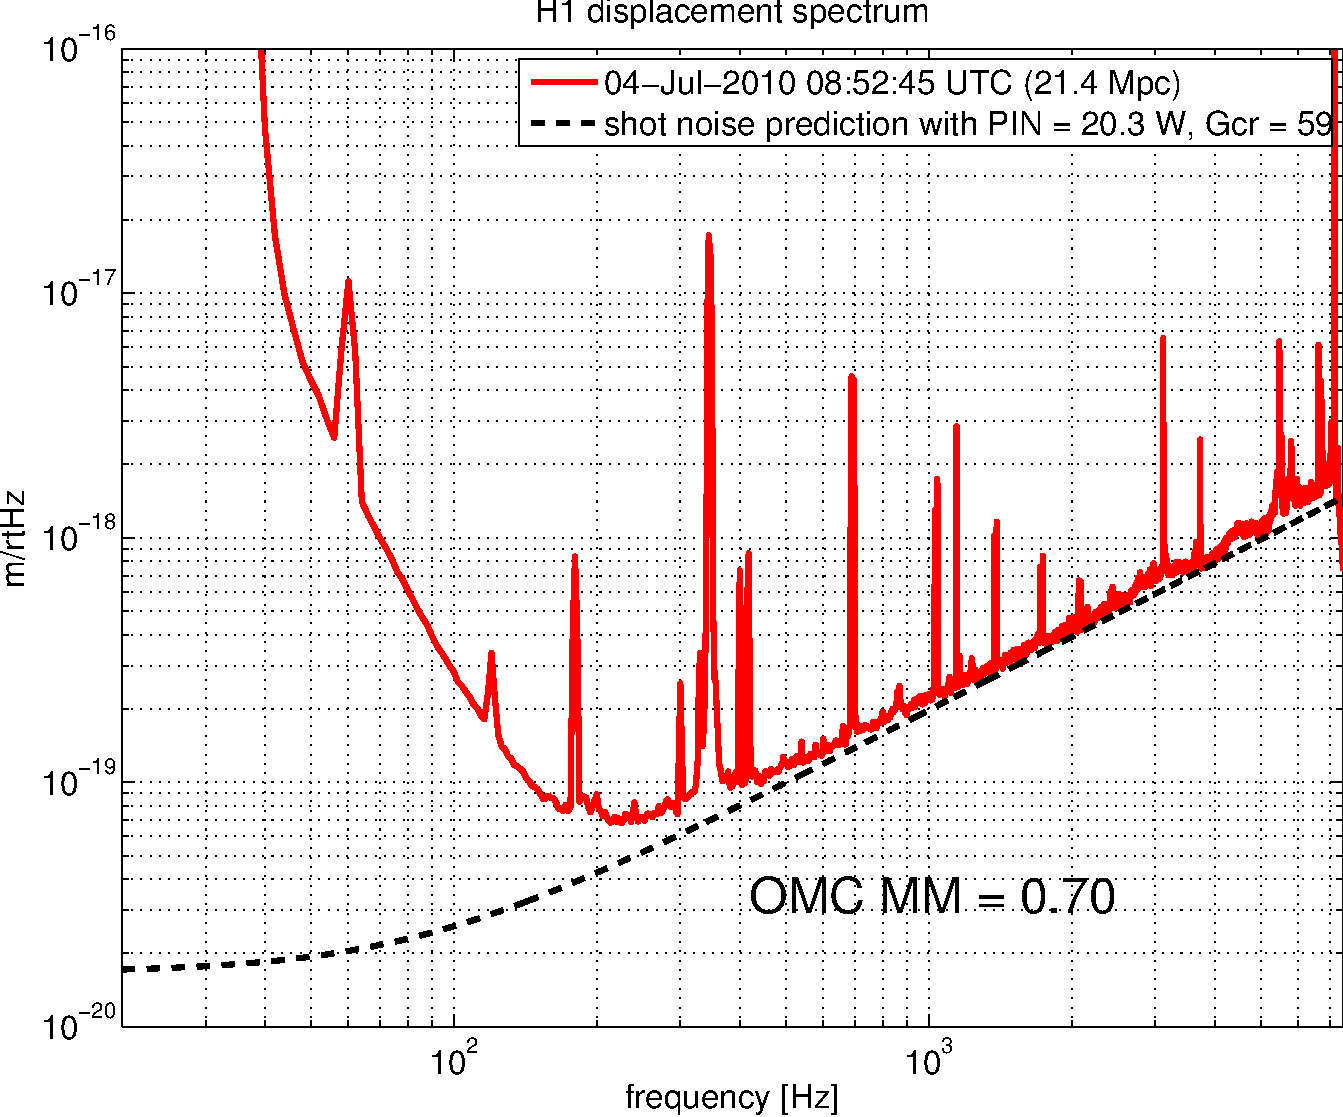
\includegraphics[width=0.45\columnwidth]{chapter5/figures/H1-962268780.pdf}
}
\subfloat[Livingston][Livingston]{
  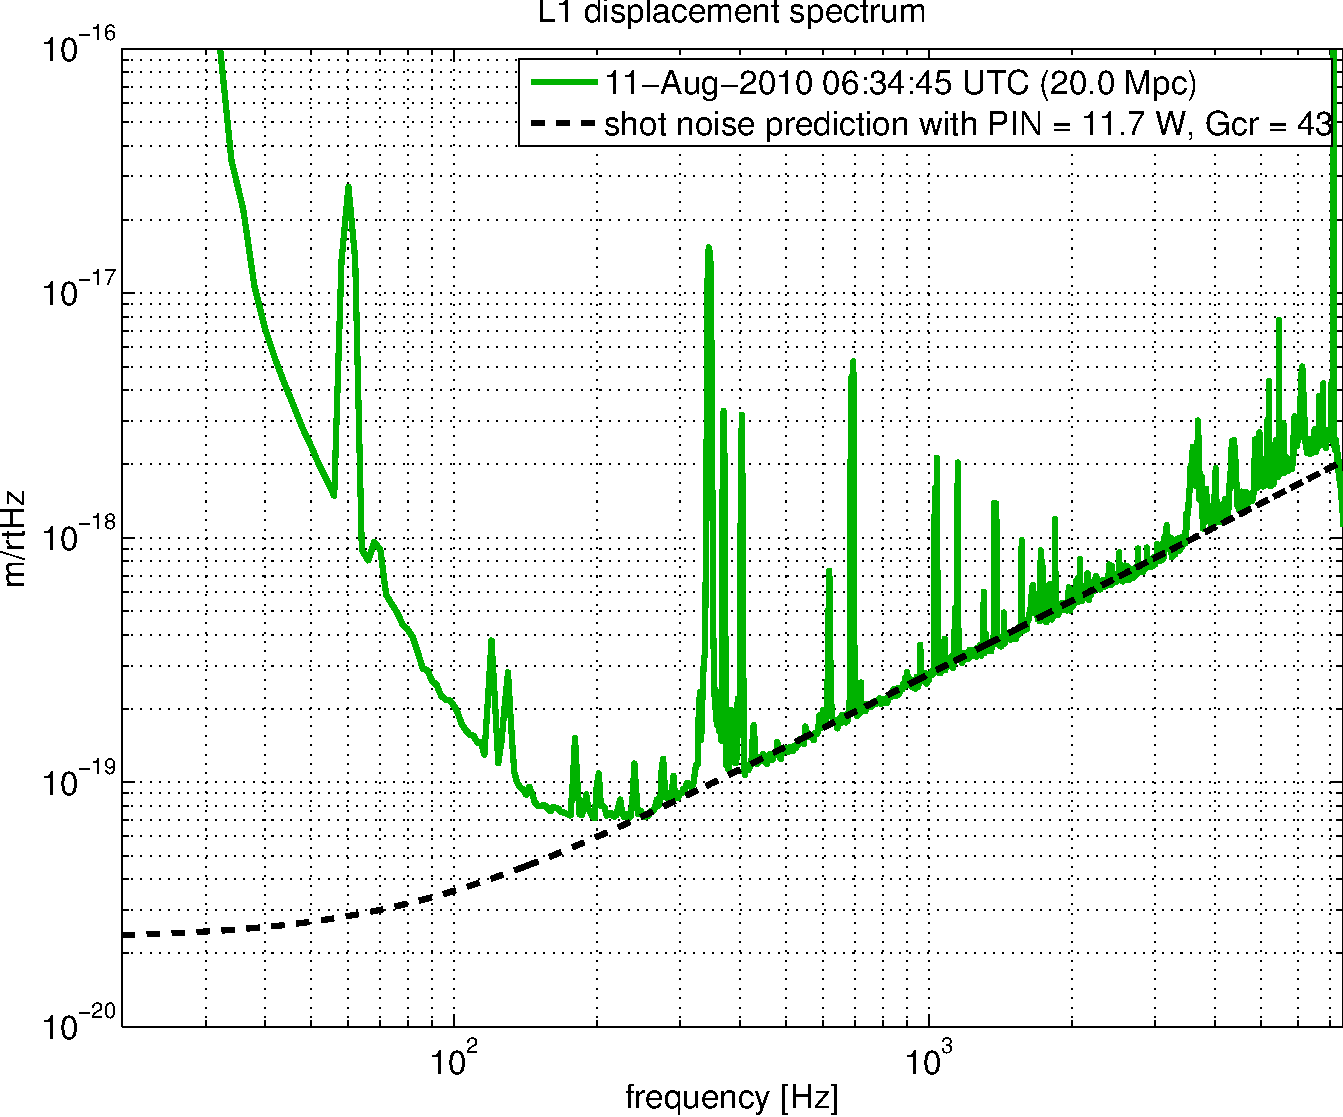
\includegraphics[width=0.45\columnwidth]{chapter5/figures/L1-965543700.pdf}
}
\caption{\label{fig:shot-noise-limited-sensitivity}Shot noise limited sensitivity of the Livingston and Hanford detectors.}
\end{figure}



%% Cavity properties [Table]
% These values are all from Sam's document T080144:
% https://dcc.ligo.org/cgi-bin/private/DocDB/ShowDocument?docid=5416
\begin{table}
\centering
\begin{tabular}{l l l l l}
\hline 
\textbf{parameter}          &\textbf{Hanford}&\textbf{Livingston}  \\
\hline
arm cavity phase gain       & 137            & 137         \\
input optics efficiency     & 0.82           & 0.75        \\
interferometer mode-matching&                & 0.92        \\
carrier recycling gain      & $59\pm6$       & 41          \\
modulation depth            & 0.34           & 0.33        \\
OMC transmission            & 0.97           &             \\
OMC mode-matching           & 0.70           & 0.95        \\
Output Faraday transmission & $0.94\pm0.02$  & 0.9805      \\
DC-readout path pickoff     & 0.953          & 0.972       \\
PD quantum efficiency       & 0.98           &             \\
\hline
\end{tabular}
\caption{Designed and measured properties of the Hanford and Livingston interferometers.}
\label{tab:ifo-properties}
\end{table}


\SECTION{Laser and Oscillator noise couplings}


For the purpose of computing the frequency response of the interferometer and
the expected laser and oscillator noise couplings, it is convenient to regard
the electric field at any given location in the interferometer as a comb of
discrete spectral lines.  Generically, we refer to any spectral line as a
`sideband'.  The sidebands are divided into radio-frequency (RF) sidebands and
audio-frequency (AF) sidebands. The distinction is not actually the frequency of
the lines but their magnitude; RF sidebands have some finite amplitude, while
audio-frequency sidebands are infinitessimal.  When the electric field is
incident upon a photodiode, the photodiode will see a beat signal between every
pair of sidebands.  In our formalism we make the approximation that the product
of any two audio-frequency sidebands is zero.  Audio-frequency sidebands are
used simply as test fields to evaluate linear transfer functions.  They produce
signals at PDs by beating against the finite-amplitude RF sidebands.

As detailed in the preceeding chapter, the state of the LIGO interferometer is
determined by sampling the electric field at various ports using photodiodes.
Pairs of RF sidebands at several distinct frequencies are introduced at the
input to the interferometer; interference between these various fields allows
the state of the interferometer to be determined.  Around the laser carrier,
there are two pairs of RF sidebands, each produced through phase modulation: the
\emph{resonant sideband} at $\sim$25 MHz, which enters the interferometer and
emerges at the output port; and the \emph{non-resonant sideband} at $\sim$61
MHz, which is mostly reflected by the power recycling mirror.

For an intuitive understanding of the noise couplings to DC readout, we will
consider only the resonant sideband, an ignore the residual non-resonant
sideband.  In numerical simulations, both are included.  The arrangement of RF
sidebands is depicted in figure~\ref{fig:af-sidebands}.

Sidebands are typically created in pairs around a modulated the parent field;
and, when incident on a photodiode, they are most conveniently treated in pairs
too.  Instead of considering the amplitudes of upper and lower sidebands
separately, we can instead use a basis where we quantify the sidebands as some
amount of amplitude modulation (AM) and some amount of phase modulation.

\begin{figure}[]
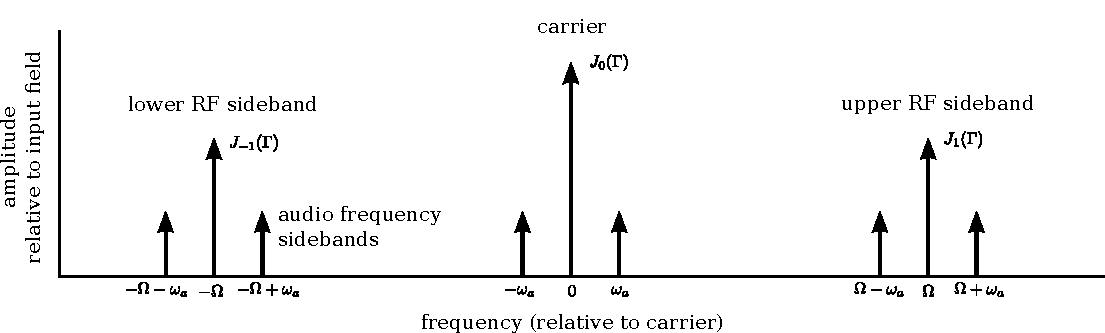
\includegraphics[width=\columnwidth]{figures/af_sidebands.pdf}
\label{fig:af-sidebands}
\caption{Schematic diagram of the laser carrier and RF sidebands, and their
  associated audio-frequency sidebands.}
\end{figure}

\SUBSECTION{Laser noises}

The Michelson-based design of laser interferometer gravitational wave detectors
is attractive due to its high common mode noise rejection.  A Michelson
interferometer with identical arms would completely isolate the output port from
common-mode noises (i.e. noise introduced at the input port).  Any asymmetries
between the arms will introduce couplings of noises at the input port to the
output port.  Some such asymmetries are unintentional, such as the difference in
finesse or reflectivity of the arms; intentional DARM and MICH asymmetries are
introduced in order to allow the local oscillator (RF or carrier) to read the
output port.

\subsubsection{Laser intensity noise}

Coupling of laser intensity noise to the output port is one of the easiest
couplings to understand.  The dominant mechanims (in the absence of radiation
pressure effects) are:
%
\begin{itemize}
\item Below the coupled-cavity pole ($f_{cc}\approx 1$ Hz), carrier power
  fluctuations are transmitted directly to the output port, attenuated only by
  the ratio $P_{AS}/P_{IN}$.  Above the coupled cavity pole, transmission of AM
  on the carrier is attenuated by $1/f$.
\item The resonant RF sidebands and any modulation they carry reaches the output
  port attenuated only slightly, since the Michelson is arranged (via the
  Schnupp asymmetry) to conduct the RF sidebands to the output port.  Because
  the RF sidebands are not resonant in the arms, noise on the RF sidebands is
  not attenuated by the coupled-cavity pole; instead they see a much lower
  finesse power recycling cavity and transmission is essentially flat in the
  band of interest.  Once reaching the output port, however, the RF sidebands
  are strongly attenuated by the OMC.
\end{itemize}
At low frequency, the carrier contribution dominates; at higher frequency the
residual RF sidebands dominate.

Laser intensity noise creates a varying radiation pressure force in the arm
cavities, which in turn causes displacement noise.  To distinguish this effect
from the inherent \emph{quantum} radiation pressure
noise\cite{Caves1980QuantumMechanical}, we refer to this as \emph{technical}
radiation pressure noise.  For identical arm cavities, the effect would be
entirely common mode.  Differences in arm cavity finesse and (especially) the
intentional differential detuning of the arm cavities produce a (potentially
large\cite{ChaibiOptomechanical}) coupling of technical radiation pressure noise
to DARM.

\subsubsection{Laser frequency noise}

\begin{figure*}[]
% Laser AM
\subfloat[Laser amplitude noise coupling (L1)][Laser amplitude noise coupling
  (L1)]{ 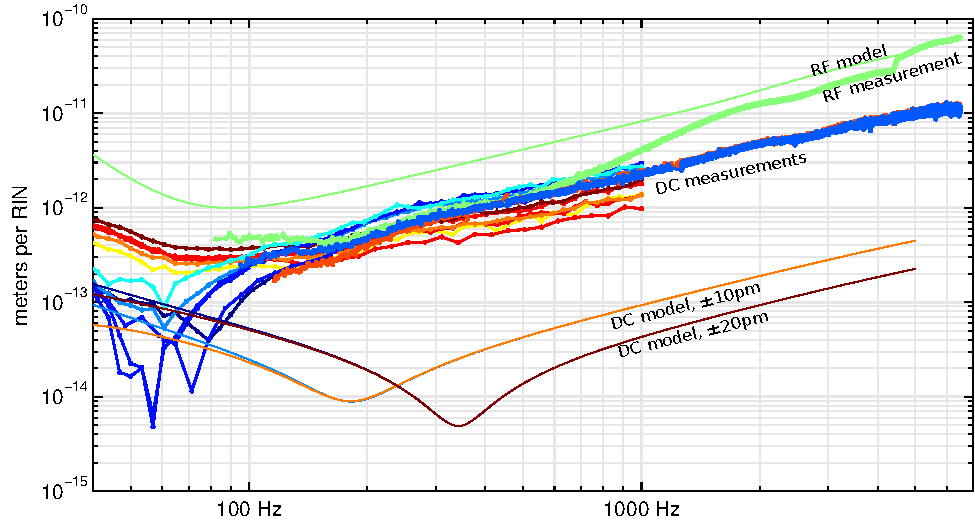
\includegraphics[]{figures/laserAM-L1.pdf}
  \label{fig:laser-AM}
}
\subfloat[Laser amplitude noise coupling (H1)][Laser amplitude noise coupling (H1)]{
  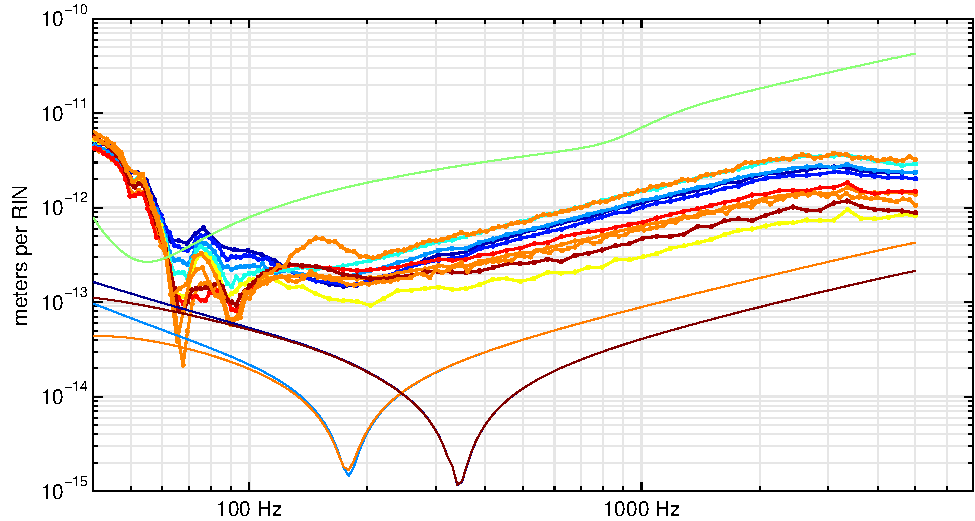
\includegraphics[]{figures/laserAM-H1.pdf}
  \label{fig:laser-AM-H1}
}

% Laser FM
\subfloat[Laser frequency noise coupling (L1)][Laser frequency noise coupling (L1)]{
  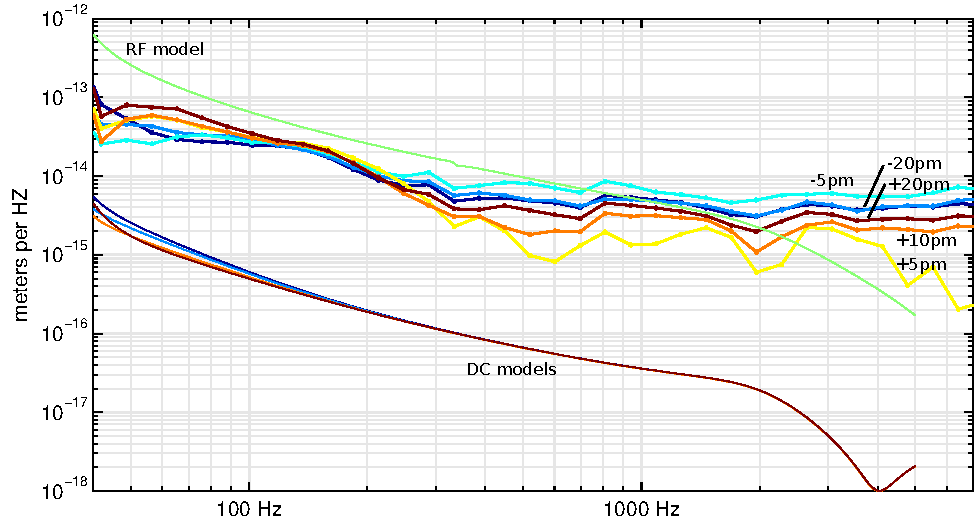
\includegraphics[]{figures/laserFM-L1.pdf}
  \label{fig:laser-FM}
}
\subfloat[Laser frequency noise coupling (H1)][Laser frequency noise coupling (H1)]{
  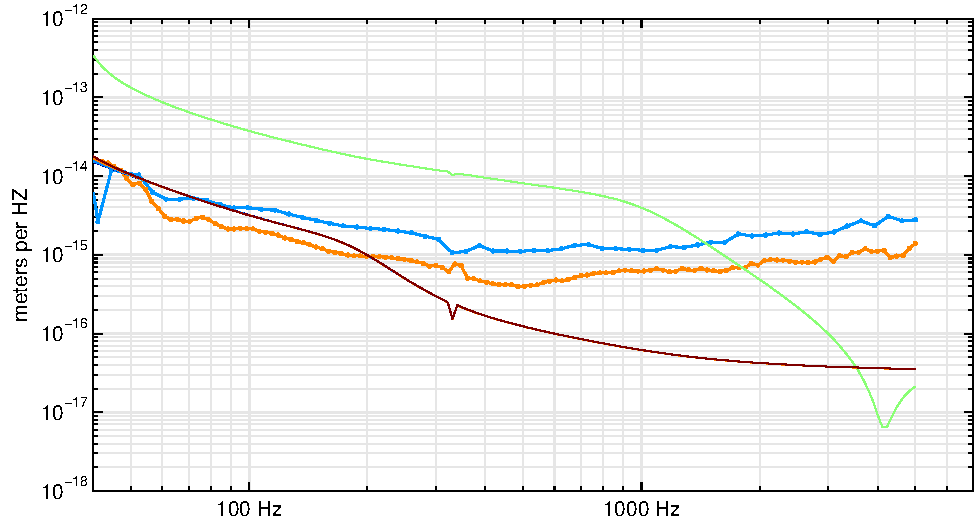
\includegraphics[]{figures/laserFM-H1.pdf}
  \label{fig:laser-FM-H1}
}
\end{figure*}


\SUBSECTION{Oscillator noises}
%
Reduced coupling of noises from the RF oscillator is one of the
motivations for implementing DC readout. Despite not relying on the RF
sidebands directly, behavior of the RF oscillator is still able to
enter into the DC readout signal through control loop cross-couplings,
leakage of RF sideband power through the OMC, and amplitude modulation
of the laser carrier induced via AM on the RF oscillator.

\begin{figure*}
% Oscillator AM
\subfloat[Oscillator amplitude noise coupling (L1)][Oscillator amplitude noise coupling (L1)]{
  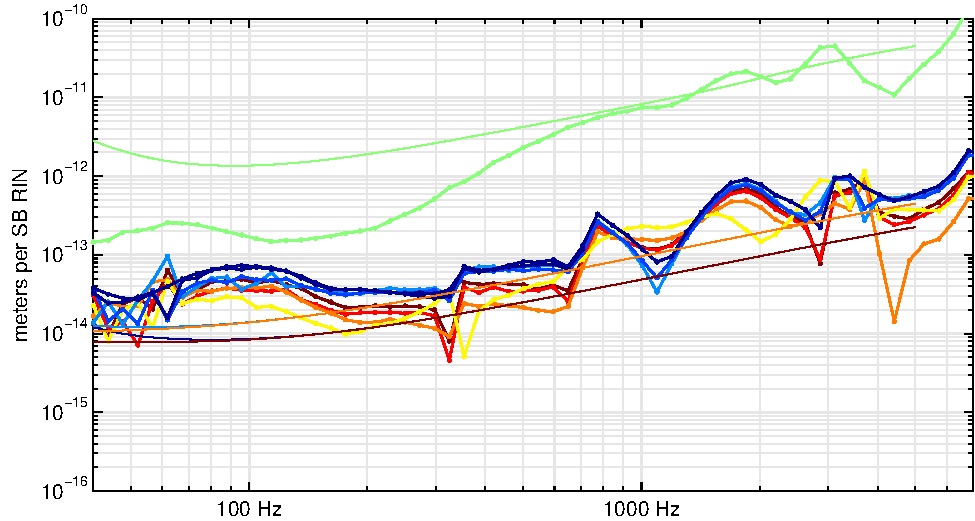
\includegraphics[]{figures/oscAM-L1.pdf}
  \label{fig:osc-AM}
}
\subfloat[Oscillator amplitude noise coupling (H1)][Oscillator amplitude noise coupling (H1)]{
  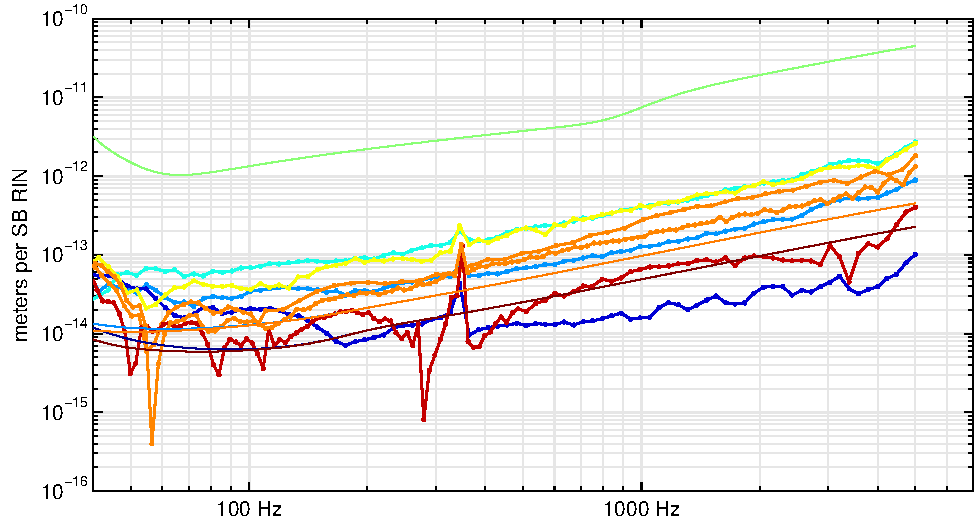
\includegraphics[]{figures/oscAM-H1.pdf}
  \label{fig:osc-AM-H1}
}

% Oscillator PM
\subfloat[Oscillator phase noise coupling (L1)][Oscillator phase noise coupling (L1)]{
  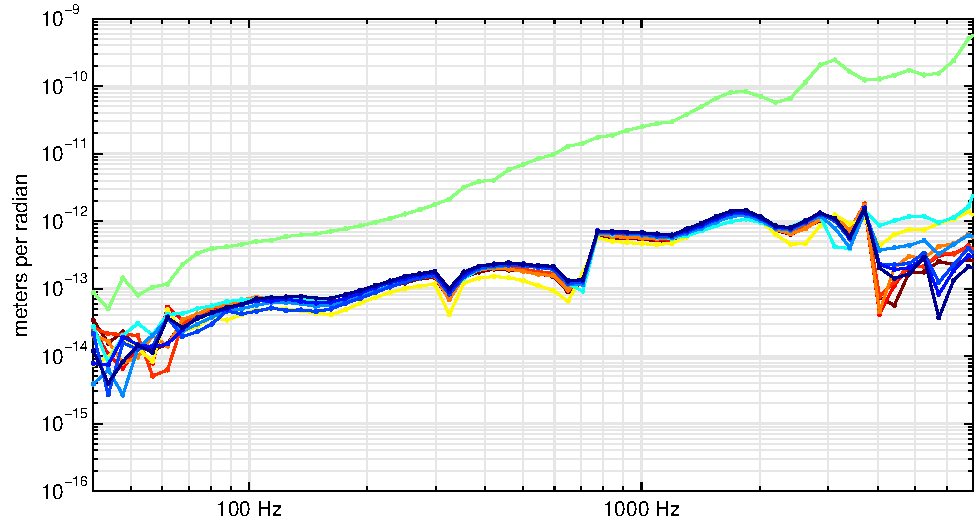
\includegraphics[]{figures/oscPM-L1.pdf}
  \label{fig:osc-PM}
}
\subfloat[Oscillator phase noise coupling (H1)][Oscillator phase noise coupling (H1)]{
  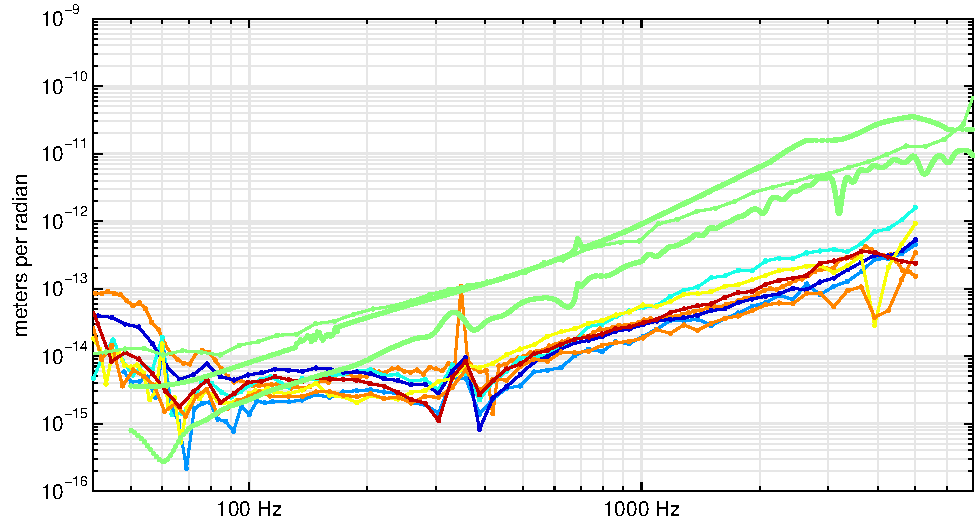
\includegraphics[]{figures/oscPM-H1.pdf}
  \label{fig:osc-PM-H1}
}

\caption{\label{noise-couplings}Oscillator and laser noise couplings to the gravitational wave readout channel, calibrated in equivalent displacement (meters).  Solid lines are the results of a frequency-domain, plane-wave model; dotted lines are linear transfer function measurements.  Color represents the DARM offset, with warm colors for positive offsets and cool colors for negative offsets.  Measurements and models for RF readout are in green.}
\end{figure*}

\subsubsection{Oscillator AM}

Amplitude fluctuations of the RF oscillator produce a fluctuating modulation
depth; when the RF oscillator signal fluctuates upwards, more power is diverted
from the carrier into the RF sidebands.  The result is somewhat similar to laser
AM, except that carrier AM and RF AM are anti-correlated instead of correlated.

Unlike laser AM, oscillator AM does not produce equal relative intensity noise
(RIN) variations of the carrier and sidebands; this is simply because oscillator
AM results in equal and opposite changes of power in the carrier and sideband
rather than linear scalings of both.  The sideband RIN per oscillator AM is
given by
\begin{equation}
\frac{\text{SB RIN}}{\text{OSC AM}}=2\Gamma_{0}\frac{J_{1}'(\Gamma_{0})}{J_{1}(\Gamma_{0})}=\Gamma_{0}\frac{J_{0}-J_{2}}{J_{1}}
\end{equation}
%(see Livingston elog 2010-07-15, {}``sideband RIN per oscillator AM calculation,'' ).
where $\Gamma_0$ is the nominal modulation depth, $J_n(z)$ is the $n$th Bessel
function, and $J_n'(z)=(\partial/\partial z)J_n(z)$ is the derivative of the Bessel function.

Measured coupling is shown in figure \ref{fig:oscillator-AM-coupling-measured}.

\subsubsection{Oscillator phase noise}

Phase noise on the RF oscillator produces phase noise on the resulting RF
sidebands, but does not affect the laser carrier.  Its direct coupling to DC
readout is therefore quite small; to couple to DC readout, the phase noise
sidebands must be converted to AM through Michelson asymmetries, and then
survive attentuation by the OMC.

Measured coupling of oscillator phase noise to the readout channel
is shown in figure \ref{fig:oscillator-PM-coupling-measured}.

\SECTION{Beam jitter noise}
%
Beam jitter noise is perhaps the most important new noise source in
DC readout and is tied to alignment of the OMC, which has proved to
be one of the most subtle new issues. The output mode cleaner converts
motion of the input beam into variations in transmission. The resulting
variation in the transmitted light level is indistinguishable from
DARM motion.



\SECTION{Electronics noise}
%
An optical power of 100 mW on the readout photodiodes will produce a
photocurrent of $i = q_e\lambda/(hc)\cdot 100\text{ mW } = 86\text{ mA}$, which
in turn has a shot noise floor of $\sqrt{2 q_e i}\approx 500 \text{
  pA}/\sqrt{\text{Hz}}$.  Across $100\ \Omega$ transimpedance, this becomes $50
\text{ nV}/\sqrt{\text{Hz}}$.  The noise floor of the readout electronics must
be below this level and not be polluted by any baseband $1/f$ flicker noise.

The main strategy is to aggressively amplify the electronic signal as close to
the photodiodes as possible, so that noises added downstream become
insignificant.  To eliminate even triboelectric effects, the first preamp stages
are placed in-vacuum.  The in-vacuum preamps consist of active filter stages
with two zeros at 8 Hz and two poles at 80 Hz, for a factor of 100 amplification
at 100 Hz.  This is followed by two more pole-zero pairs in satellite amplifiers
on the floor outside the vacuum chamber, for a total gain of 10,000 before the
long run to the racks.

\begin{comment}
h = 6.626068e-34;
c = 299792458;
lambda = 1064e-9;
qe = 1.60217646e-19;
I = qe * lambda / (h * c)
sqrt(2* qe * I)
\end{comment}

\SECTION{Optical spring}
%
Detuning the arm cavities from their resonance introduces a big optical
spring.

\begin{equation}
k_{opt}\approx\frac{64\mathcal{F}^{2}g^{2}P_{IN}}{c\lambda^{2}}\left(\delta x\right) 
\end{equation}

\SECTION{Technical radiation pressure noise}

Amplitude noise on the input laser field produces modulation radiation
pressure on the optics, in particular in the arm cavities.  If the arm
cavities were identical, this coupling would be entirely common mode.
However, once the arms are differentially detuned, the radiation
pressure noise attains a differential component.

We can treat the radiation pressure noise as a displacement noise.

Suppose the arm cavities are initially identical, with all 
suspensions having resonant frequency $\omega_0$.  The optical spring
shifts this resonance to $\omega_0 \pm \delta\omega$.

The intensity noise to displacement transfer function is
\begin{equation}
  P_{IN} {g_{rc}}^2 {g_{cav}}^2 \frac{1}{s_{cc}} 
\end{equation}

\SECTION{Nonlinearity  of the DC error signal}
%
Although we operate sufficiently far from the dark fringe that the
linear coupling of residual DARM motion to output power is dominant,
sufficiently large motion could produce second-order coupling. Fortunately,
this turns out to be totally negligible.

\SECTION{Noise budget}
\SECTION{Optical gain}

\SECTION{Digital effects}

The realtime digital signal processing system through which our
control systems are implemented provide the illusion of a continuous,
analog system.  However, it is important to remember that the
underlying system operates on quantized values in discrete time in
order to avoid being caught by surprise by ``digital noises''.

\begin{itemize}
\item Finite, non-deterministic execution time
\item ADC bit noise
\item Floating point dynamic range
\item Synchronized communications
\end{itemize}

\CHAPTER{Conclusion}
\label{conclusion}

Over the last several decades, the state of the art of gravitational
wave detection has advanced to the point where we are likely to
discover gravitational waves with the detectors currently under
construction.

Enhanced LIGO successfully demonstrated the viability of DC readout as
a low noise interferometer readout technique.  The DC readout system
(including the output mode cleaner) in Enhanced LIGO alleviated the
problems experienced with the heterodyne readout in initial LIGO,
allowed us to increase the interferometer input power (increasing the
detectors' sensitivity), and delivered the expected shot-noise-limited
performance.  The dual Enhanced LIGO goals of both increasing the
detector sensitivity and gaining early experience with Advanced LIGO
technologies were achieved.

During Enhanced LIGO we identified OMC alignment as a particularly
important and unexpectedly subtle aspect of the OMC system, and
identified and implemented an effective alignment system.  We also
gained valuable experience in the mitigation of beam jitter coupling.

Measurements of the couplings of laser and oscillator noises reveal
that the couplings are generally improved over RF readout.  Comparison
of measured laser noise couplings with simple plane-wave models
reveals that more sophisticated models (most likely incorporating
higher-order spatial modes) are necessary to explain the measured
couplings.  The effect of spurious higher order modes will be
mitigated in Advanced LIGO through the use of geometrically stable
cavities, better optics, and improved thermal compensation; however,
to the extent that the design relies on achieving the noise couplings
predicted by a simple plane-wave model, I expect a long period of
commissioning in order to achieve it.  




\appendix
\CHAPTER{Table of Abbreviations}
\label{chapter6}
\section{Abbreviations}
\singlespacing
\begin{tabular}{|l|l|}
\hline 
AF   & audio frequency \\
AM   & amplitude modulation \\
AS   & antisymmetric (output) port \\
ASC  & angular sensing and control \\
BS   & beamsplitter \\
CARM & common arm length \\
CM   & common mode \\
DARM & differential arm length; the gravitational wave readout channel \\
DC   & direct current (i.e. zero frequency) \\
ETM  & end test mass \\
FSR  & free spectral range \\
FWHM & full width, half max \\
GW   & gravitational wave \\
IFO  & interferometer \\
ISC  & interferometer sensing and control \\
ISS  & intensity stabilization servo \\
ITMX & input test mass, X arm \\
LHO  & LIGO Hanford Observatory \\
LIGO & Laser Interferometer Gravitational-wave Observatory \\
LLO  & LIGO Livingston Observatory \\
LSC  & length sensing and control \\
LSC  & LIGO Scientific Collaboration \\
MC   & mode cleaner \\
MICH & Michelson interferometer \\
OMC  & output mode cleaner \\
PD   & photodiode \\
PM   & phase modulation \\
PRC  & power recycling cavity \\
PSL  & pre-stabilized laser \\
RF   & radio frequency \\
RIN  & relative intensity noise $(\delta P/P)$ \\
SNR  & signal-to-noise ratio \\
\hline
\end{tabular}

\section{symbols}

\begin{tabular}{|l|l|}
\hline
$\nu_0$         & free spectral range \\
$f$             & frequency (Hz) \\
$f_c$           & cavity pole \\
$\mathcal{F}$   & arm cavity finesse \\
$g_\phi$         & phase gain \\
$s$             & Laplace parameter ($s=i\omega$) \\
$\omega$        & angular frequency ($\omega=2\pi f$) \\
$L$             & cavity length \\
$\nu$           & optical frequency (Hz) \\
\hline
\end{tabular}

\include{ligodesign/ligodesign}
\chapter{Fabry-Perot cavities}
\label{sec:cavities}
In this appendix I derive the basic properties of Fabry-Perot
cavities~\cite{Fabry1892Theorie,Fabry1901New} in the plane wave approximation.
Excellent references with further detail include \cite{Siegman1990Lasers}, \cite{Fox1961Resonant},
and the general optics reference \cite{Haus1983Waves}.

%\cite{Butler2004Characterization}
\subsection{Fabry-Perot field equations}

\begin{figure}
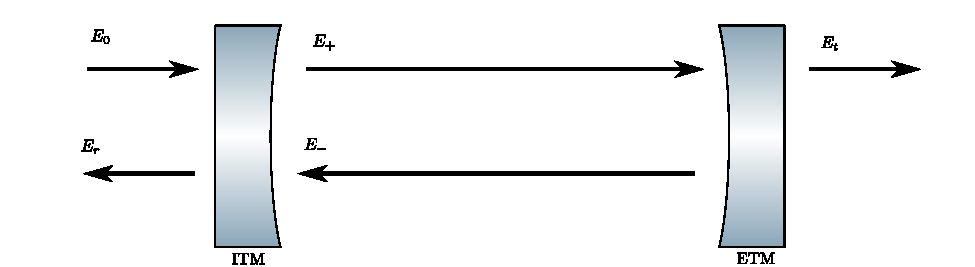
\includegraphics[]{figures/cavity.pdf}
\caption[Fabry-Perot Cavity]{\label{fig:fabry-perot}Fabry-Perot
  cavity.  When used as an arm cavity, the two mirrors are known as
  the input (ITM) and end (ETM) test masses.  Here $E_0$ indicates the
  amplitude of the incident electric field, $E_r$ the reflected field,
  $E_+$ the forward-going intra-cavity field, etc.}
\end{figure}

We begin by writing down the relationships between the fields at each
interface.  For simplicity, we treat each mirror as a single (thin)
interface.  Let $r_1$ and $t_1$ be the amplitude reflectivity and
transmissivity for the input mirror, and $r_2$ and $t_2$ describe the
output mirror.  I use the phase convention where transmission through
a mirror conveys $90^\circ$ of phase, i.e. a factor of $i$ in the
amplitude:
%
\begin{align}
E_+ &= i t_1 E_0 + r_1 E_- \\
E_- &= r_2 e^{i 2 \phi} E_+ \\
E_t &= i t_2 e^{i \phi} E_+ \\
E_r &= r_1 E_0 + i t_1 E_1
\end{align}
%
Solving these equations algebraically for $E_r$ and $E_t$ in terms of the incident field $E_0$, we find the transmission and reflectivity of the cavity:
%
\begin{align}
t_c \equiv & \frac{E_t}{E_0} = 
         \frac{-t_1 t_2 \exp i\phi}
              {1 - r_1 r_2 \exp i2\phi} \\
r_c \equiv & \frac{E_r}{E_0} = 
         \frac{r_1 - \left({r_1}^2 + {t_1}^2\right)r_2 \exp{i2\phi}}
              {1 - r_1 r_2 \exp i2\phi}
\label{eq:cavity-reflectivity}
\end{align}
%
where $\phi=(2\pi/\lambda)L$ is the phase accumulated by the field as it travels from
the first mirror to the second mirror.  This phase depends on both the
laser wavelength and the distance between the mirrors:\footnote{There is an additional contribution to the phase, the Guoy phase shift, due to geometric effects; this is described in chapter 4.  Also note that some references use the \emph{round-trip} phase rather than the \emph{one-way} phase used here.}
\begin{align}
\phi  & = \pi (\nu / \nu_0) \\
\nu_0 & = c/(2L)
\end{align}
where $\nu=c/\lambda$ is the laser frequency, $L$ is the cavity
length, and $\nu_0$ is the \emph{free spectral range}, which describes
the spacing between adjacent resonances.

\subsection{the cavity pole}
It is often useful to write the cavity reflectivity in the form of a
rational transfer function,
\begin{equation}
r_c(s) = \prod_{n=-\infty}^{\infty} \frac {s-z_n} {s-p_n}
\label{eq:rational-function}
\end{equation}
where $s=i\omega$, $\{z_n\}$ are the zeroes of $r_c(s)$, and $\{p_n\}$
are the poles.  To find the poles and zeroes, make the substitution
$\phi=-is/(2\nu_0)$ and solve for the zeroes of the numerator and
denominator of equation~\ref{eq:cavity-reflectivity} separately.  We find:
\begin{align}
p_n &= - \omega_{fsr} \left(\log\left(r_1 r_2\right) +  i n\right)  & \forall n\in \mathbb{Z}\\
z_n &= + \omega_{fsr} \left(\log\left(r_1/r_2\right) +  i n\right)  & \forall n\in \mathbb{Z}
\end{align}
where $\omega_{fsr}\equiv2\pi\nu_0$.

Because this function is periodic in $i\omega$, we can in many
circumstances regard the laser carrier as having a frequency
$\nu=0$ rather than $\nu = n\nu_0$ for some very large $n$.

\begin{figure}
\centering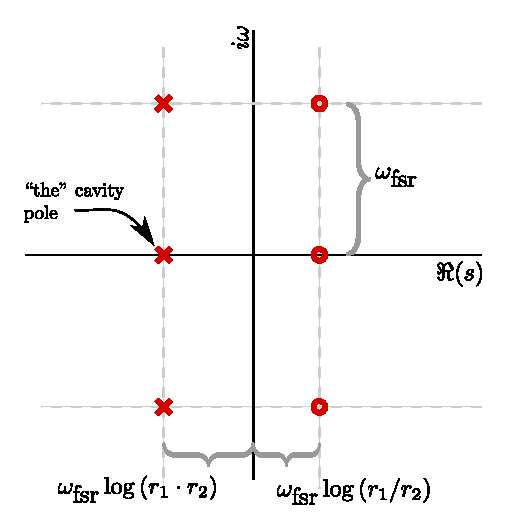
\includegraphics{figures/cavitypzmap.pdf}
\caption[Pole-zero map of Fabry-Perot cavity reflectivity]{\label{fig:cavpzmap} Pole-zero map of the cavity amplitude
  reflectivity.
  Poles are designated with $\times$ and zeros with
  $\circ$; $r_1$ is the amplitude reflectivity of the input coupler,
  and $r_2$ is the amplitude reflectivity of the output coupler.
  Losses can be lumped into $r_2$.  Notice that the free spectral
  range (angular frequency $\omega_{\textrm{fsr}}$) sets the scale of
  the entire diagram, and the function is periodic in $i\omega$: there
  is an infinite line of poles and an infinite line of zeros.  Two
  limiting cases are worth considering: (1) A critically-coupled
  cavity has $r_1=r_2$, which brings the line of zeros onto the
  imaginary axis. On resonance, $i\omega$ travels through these zeros
  and the cavity reflectivity vanishes.  This models the desired
  behavior of mode cleaner cavities. (2) A maximally over-coupled
  cavity has $r_2=1$, in which case the line of poles and line of
  zeros are equally spaced from the imaginary axis.  This models the
  LIGO arm cavities.  
  The cavity's amplitude transmission has the same poles as the
  reflectivity but no zeros.
}
\end{figure}

\subsection{phase gain}
Our interest in using Fabry-Perot cavities as the arms of a
gravitational wave detector is in having the light traverse the length
of the arm multiple times, multiplying the effect of any optical path
length perturbations caused by a GW.  We can derive the magnitude of
this \emph{phase gain} by examining how the phase of the light reflected from
the cavity changes as the intra-cavity phase $\phi$ changes, for small
variations from resonance.

Suppose $z(t)=A(t) \exp\{i \phi(t)\}$ is an arbitrary complex-valued
function with amplitude $A(t)$ and phase $\phi(t)$. By taking the
logarithm before taking the derivative, we can separate the amplitude
and phase:
%
\begin{equation}
\frac{\partial}{\partial t} \log z(t) = \left(\frac{\partial}{\partial t} \log A(t)\right) + i \left(\frac{\partial}{\partial t} \phi(t)\right)
= \frac{1}{z(t)} \frac{\partial}{\partial t} z(t)
\end{equation}
%
This gives us an expression for the rate of change of the phase of a function:
%
\begin{equation}
\frac{\partial}{\partial t} \arg z(t) = \text{Im} \frac{1}{z(t)} \frac{\partial}{\partial t} z(t)
\end{equation}

We can find the phase gain of a Fabry-Perot cavity by applying this expression to the cavity reflectivity as a function of intra-cavity phase, $r_c(\phi)$:
\begin{equation}
g_\phi = \text{Im\ } \frac{r_c'}{r_c}
\end{equation}
where $r_c'(\phi)\equiv(1/2)(\partial/\partial\phi)r_c(\phi)$; the factor of $1/2$ is to convert from round-trip phase to one-way phase.  Because the derivative of the amplitude of $r_c$ vanishes on resonance, we can simply take the magnitude of $r_c'/r_c$ rather than the imaginary part. Explicitly taking the derivative of equation~\ref{eq:cavity-reflectivity}, we find
\begin{equation}
r_c'(\phi) = \frac{1}{2}\frac{d}{d\phi} r_c(\phi) = 
-i \frac{\left(1-{r_1}^2\right) r_2 \exp 2 i \phi}
     {\left(1 - r_1 r_2 \exp 2 i \phi\right)^2}\\
\end{equation}
%
Conventionally the symbol $r_c'$ (as in \cite{LigoFreqResponse97}) indicates the magnitude of this expression at resonance ($\phi=0$):
\begin{equation}
r_c' = 
 \frac{\left(1-{r_1}^2\right) r_2 }
     {\left(1 - r_1 r_2 \right)^2}
\end{equation}

Another way to calculate the phase gain is to use the rational transfer function expression, equation~\ref{eq:rational-function}.  To model the situation near resonance, we need only consider the nearest pole and zero:
\[
r_c(s) \approx \frac{s - z_0}{s - p_0}
 = \frac{s - \omega_{fsr}\log \left(r_1 / r_2\right)}
        {s + \omega_{fsr}\log \left(r_1 \cdot r_2\right)}
\]
Recall that the phase at frequency $\omega$ imparted by a pole at
frequency $\omega_c$ is $\arctan\left(-\omega/\omega_c\right)$; a zero
at the same frequency subtracts this same phase.  For a maximally
over-coupled cavity (i.e. with $r_2 = 1$), the cavity pole and cavity
zero are equal and opposite, so contribute equal phase ($\arctan$ is
odd).  Use $\omega = 2\nu_0\phi$ to express the detuning phase $\phi$
as an equivalent detuning frequency.

Changing the one-way phase of the arm by $\phi$ results in a phase 
change of
\begin{equation}
\phi_r   = 2 \tan^{-1} \left( 2 \nu_0 \frac{\phi}{\omega_c} \right)
%   = 2 \tan^{-1} \left( \frac{2}{\pi}\mathcal{F}\phi\right)
\end{equation}
where $\omega_c\equiv2\pi f_c$ is the cavity pole and $\mathcal{F}=(1/2)(\nu_0/f_c)$ is the cavity finesse (which will be introduced in section~\ref{sec:finesse}).  Taking the derivative, we find the phase gain:
\begin{equation}
g_\phi =  \frac{1}{2} \frac{d \phi_r}{d \phi} 
= \frac{2 \nu_0}{\omega_c} \left[1 + \left(\frac{2 \nu_0 \phi}{\omega_c}\right)^2 \right]^{-1} 
= \frac{2 \mathcal{F}}{\pi} \left[1 + \left(\frac{\omega}{\omega_c}\right)^2 \right]^{-1} 
\end{equation}
The phase gain on resonance is $2 \nu_0 / \omega_c = 2\mathcal{F}/\pi \approx 140$. This phase gain decreases as we detune the cavity further from resonance, but it is not seriously diminished until the cavity detuning approaches the cavity pole.

\subsection{intra-cavity power buildup}

The power buildup in the cavity is given by 
\begin{equation}
\frac{P_+}{P_{IN}} = \frac{|E_+|^2}{|E_0|^2} = \frac{ T_1}{1 - 2 r_1 r_2 \cos 2\phi+\left(r_1 r_2\right)^2 }
\end{equation} 
which may be re-written (using the identity $\cos2\phi = 1 -
2\sin^2\phi$) as
\begin{equation}
\label{cavity_buildup_eq}
\frac{P_+}{P_{IN}} = \frac{g^2}{1 + F \sin^2 \phi} 
\text{  with  } F = \frac{4 r_1 r_2}{(1 - r_1 r_2)^2}
\text{  and  } g = \frac{t_1}{1-r_1 r_2}
\end{equation} 
where $F$ is the \emph{coefficient of finesse} and $g$ is the
\emph{amplitude gain}.

The form of this expression is often referred to in the literature as
an Airy function, though it is distinct from the well-known special
function of the same name.  Making the small angle approximation
$\sin\phi\approx\phi$ we see that each resonance is locally Lorentzian.

\subsection{finesse ($\mathcal{F}$)}
\label{sec:finesse}
The tightness of the resonance is quantified as the
\emph{finesse} ($\mathcal{F}$), which is defined as the ratio of the
cavity free spectral range to the full-width-half-max of the
resonance,
\begin{equation}
\mathcal{F} \equiv \frac{\nu_0}{\nu_{\mathrm{FWHM}}}
= \frac{1}{2}\frac{\nu_0}{f_c}
\end{equation}
%
where the FWHM is given by twice the cavity pole ($f_c$).  The finesse is related to the coefficient of finesse ($F$) by
%
\begin{equation}
\mathcal{F} = \frac{\pi}{2} \frac{1}{{\sqrt{\arcsin (1/F)}}} \approx \frac{\pi}{2}\sqrt{F}
\end{equation}where the approximation holds for high-finesse cavities.

The finesse ($\mathcal{F}$) of an optical cavity is analogous to
the quality factor (Q) of an oscillator. The Q factor is the ratio
of the frequency of an oscillator to its full-width-half-max bandwidth;
to compute finesse, the free spectral range (spacing between resonances)
is used instead of the oscillator frequency.

\begin{figure}
\begin{centering}
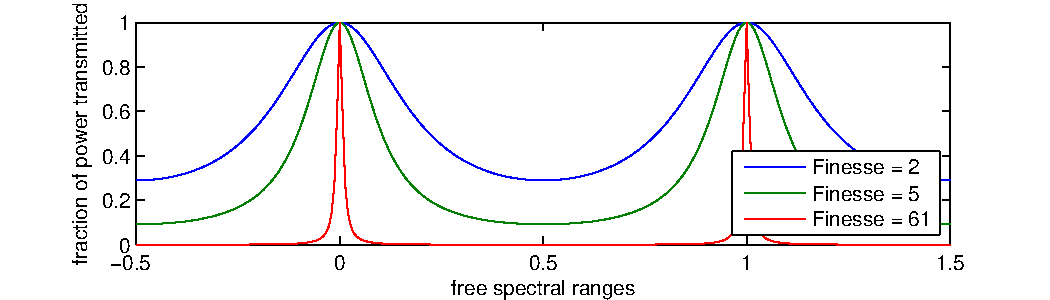
\includegraphics{figures/finesses}
\end{centering}
\caption[Cavity buildup versus detuning]{Power transmission coefficients for three critically-coupled cavities.}
\end{figure}

\subsection{Impedance matching}

From the point of view of a beam incident upon a cavity, the cavity is
either under coupled, critically coupled, or over coupled. This
coupling is determined by the comparison of the transmissivity of the
input coupler compared to all other losses in the system. For a
two-mirror, lossless cavity, the cavity is under coupled if $t_1 <
t_2$, critically coupled if $t_1 = t_2$, and over coupled if $t_1 >
t_2$.

%For a discussion of impedance in acoustic context, see \cite{Blackstock2000Fundamentals}.

\begin{figure}
\subfloat[Critically coupled cavity. Note that $r=0$ on resonance. Cavities
of this type are used as filter cavities.]{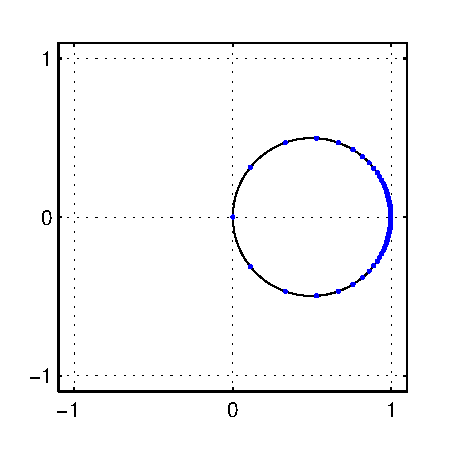
\includegraphics{figures/circles-critically-coupled}}\hfill \subfloat[Maximally over-coupled cavity. Note that $r=-1$ on resonance. Cavities
of this type are used for the LIGO arms.]{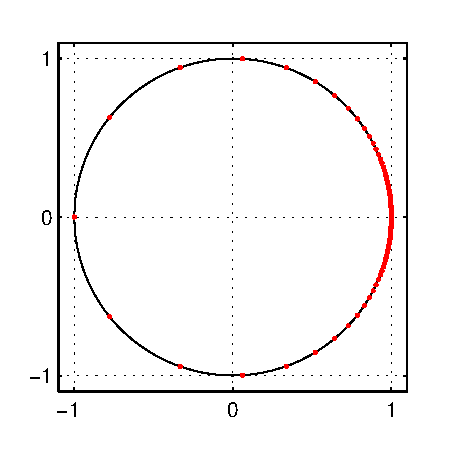
\includegraphics{figures/circles-over-coupled}}\caption[Cavity amplitude reflectivity plotted in the complex plane]{Reflection coefficients for two cavities, plotted on the complex plane,
over a free spectral range $0\leq\phi<\pi$. The x axis represents
the real part, and the y axis the imaginary part of the cavity reflection
coefficient. The dots are spaced with uniform $\Delta\phi$. They
appear more closely spaced when the phase of the cavity reflectivity
changes slowly; they appear sparsely spaced where the reflected phase
changes quickly, as the cavity goes through resonance.}
\end{figure}

\subsubsection{Critically-coupled cavities}

Maximum power is transfered into a critically coupled cavity; no power
is reflected. In this case, the prompt reflection from the input coupler
is exactly canceled by an equal-amplitude, opposite-phase leakage
beam from the field inside the cavity. Because an (ideal) critically
coupled resonator is perfectly transmissive for light at the resonant
frequency, they are used as filter cavities.

The transmission of power through a filter cavity may be found by
multiplying equation \ref{eq:powerbuildup} by the output coupler
power transmissivity $T={t_{1}}^{2}={t_{2}}^{2}$: 
\begin{equation}
T_{c}=\frac{1}{1+F\sin^{2}\phi}=\begin{cases}
1 & \text{at resonance (maximum transmission)}\\
1/(1+F) & \text{at anti-resonance (minimum transmission)}
\end{cases}
\end{equation}
where we see that the (coefficient of) finesse quantifies the attenuation
of non-resonant modes (in addition to the width of the resonance).

The power buildup inside a critically-coupled two-mirror cavity is
simply the inverse of the mirror transmission:
\[
g^{2}=\left(\frac{t_{1}}{1-r_{1}r_{2}}\right)^{2}=\frac{t^{2}}{\left(1-r^{2}\right)^{2}}=\frac{1}{T}
\]
This can also be seen from a very simple argument: if the power emerging
from the output coupler is equal to $P_{IN}$, then the power inside
the cavity must be $P_{IN}/T$.


\subsubsection{Over-coupled cavities}

The LIGO arms are strongly over-coupled cavities. A lossless maximally over-coupled
cavity (i.e. with $t_{2}=0$) acts as a perfect reflector. 

For high-finesse, highly-overcoupled cavities, the cavity power buildup
$g^{2}$ is approximately equal to the square root of the coefficient
of finesse, or $(2/\pi)$ times the finesse:
\begin{equation}
g^{2}\approx\sqrt{F}\approx\frac{2}{\pi}\mathcal{F}
\end{equation}
This can be seen by setting $r_{2}=1$ and using $\sqrt{x}\approx1+(x-1)/2$
for $x\approx1$:
\begin{equation}
g^{2}\bigg|_{r_{2}\to1}=\frac{1-r_{1}^{2}}{\left(1-r_{1}\right)^{2}}=\frac{1+r_{1}}{1-r_{1}}\approx\frac{2\sqrt{r_{1}}}{1-r_{1}}=\sqrt{F}\bigg|_{r_{2\to1}}
\end{equation}
%
%
Another useful approximation is:
\[
g^{2}\approx\frac{4}{T_{1}}
\]

\chapter{The Optical Spring}
When detuned from resonance, the power circulating within a Fabry-Perot
cavity varies linearly with small deviations from that detuning. This
gives rise to a displacement-dependent force, which can be described
via a spring constant. This effect is called the \emph{optical spring}
\footnote{This is the longitudinal optical spring; an \emph{angular} optical spring
also arises, due to interactions between off-center radiation pressure and cavity geometry~\cite{Sidles2006Optical}.}.  Optical springs has been observed and studied in several experiments~\cite{Sheard2004Observation}.

For frequencies that are slow compared to the cavity pole, we can
calculate the behavior of the spring using a quasi-static approximation,
simply using the derivative of the power buildup versus cavity detuning.

The power circulating in a cavity is:
\begin{equation}
\frac{P_{+}}{P_{IN}}=\frac{g^{2}}{1+F\sin^{2}\phi}
\end{equation}
where $P_{IN}$ is the incident power, $P_{+}$ is the forward-circulating
power, $g^{2}=\left(t_{1}\right)^{2}/\left(1-r_{1}r_{2}\right)$ is
the power buildup on resonance, $F=4r_{1}r_{2}/\left(1-r_{1}r_{2}\right)^{2}$
is the coefficient of finesse%
\footnote{The finesse ($\mathcal{F}$) is related to the coefficient of finesse
($F$) via $\mathcal{F}\approx\frac{\pi}{2}\sqrt{F}$.%
}, and $\phi$ is the one-way phase detuning of the cavity, which is
related to cavity length $x$ as $\phi=(2\pi/\lambda)x$. 

For a given power circulating in the cavity, the radiation pressure
force due to the intra-cavity power on each of the mirrors is $f=2P/c$.
We can find the spring constant by taking the derivative:

\[
k\equiv-\frac{\partial f}{\partial x}=-\frac{\partial}{\partial x}\frac{2P}{c}=-\frac{2}{c}\frac{\partial\phi}{\partial x}\frac{\partial P}{\partial\phi}
\]
Working out the derivative, we find:

\begin{align}
\frac{\partial}{\partial\phi}P_{+} & =-2Fg^{2}\frac{\cos(\phi)\sin(\phi)}{\left(1+F\sin^{2}\phi\right)^{2}}P_{IN}\\
 & =-2Fg^{2}P_{IN}\phi+O\left(\phi^{3}\right)
\end{align}
Putting it all together, we get:
\begin{align}
k & =2Fg^{2}\left(\frac{2P_{IN}}{c}\right)\left(\frac{2\pi}{\lambda}\right)\frac{\cos(\phi)\sin(\phi)}{\left(1+F\sin^{2}\phi\right)^{2}}\label{eq:spring-constant}\\
 & \approx2Fg^{2}\left(\frac{2P_{IN}}{c}\right)\left(\frac{2\pi}{\lambda}\right)\frac{\phi}{\left(1+F\phi^{2}\right)^{2}}\label{eq:spring-constant-approx1}\\
 & \approx2Fg^{2}\left(\frac{2P_{IN}}{c}\right)\left(\frac{2\pi}{\lambda}\right)\phi+O\left(\phi^{3}\right)
\end{align}


where, of course, $\phi=(2\pi/\lambda)\delta x$, where $x$ is the
(one-way) detuning length. If a mirror is displaced by $(\delta x)$,
the spring constant is:
\[
k\approx\frac{64\mathcal{F}^{2}g^{2}P_{IN}}{c\lambda^{2}}\left(\delta x\right)
\]
Putting in some numbers for the Enhanced LIGO arms:
\begin{align*}
\mathcal{F} & =220\\
g^{2} & =137\\
P_{IN} & =400\mathrm{\ Watts}\\
\lambda & =1064\mathrm{\ nm}\\
\delta x & =5\mathrm{\ pm}\\
\hline k & \approx2500\mathrm{\ N/m}
\end{align*}
For comparison, the mechanical restoring force has a spring constant
of approximately
\[
k_{m}=m\omega^{2}\approx\left(10.5\text{ kg}\right)\left(2\pi\cdot0.7\text{5 Hz}\right)^{2}\approx230\text{ \ensuremath{\frac{\text{N}}{\text{m}}}}
\]


It can also be handy to put Eq. \ref{eq:spring-constant-approx1}
into terms of the unitless detuning parameter $\delta_{\gamma}=\sqrt{F}\phi$,
where $\delta_{\gamma}\equiv\frac{\delta}{\gamma}$, where $\delta$
is the cavity detuning (in radians/sec), and $\gamma$ is the line-width
(cavity pole) in the same units. If we further assume that the cavity
is strongly-overcoupled, we can use the relations $g^{2}=\sqrt{F}=\frac{2}{\pi}\mathcal{F}=4/T_{1}$.
With these substitutions (and $\lambda=2\pi c/w_{0}$), we recover
expression (3.14) given in Thomas Corbitt's thesis \cite{Corbitt2008Quantum}:
\begin{equation}
K_{0}\approx\frac{64P_{IN}w_{0}}{T^{2}c^{2}}\frac{\delta_{\gamma}}{\left(1+\delta_{\gamma}^{2}\right)^{2}}
\end{equation}


\section*{Coupled oscillators}

Consider a system of two masses, connected to each other via a spring
with spring constant $k_{1}$ and each connected to the wall via a
spring of spring constant $k_{0}$. (Later, $k_{0}$ will represent
the pendula by which the optics are suspended, and $k_{1}$ will represent
the optical spring.)

\begin{center}
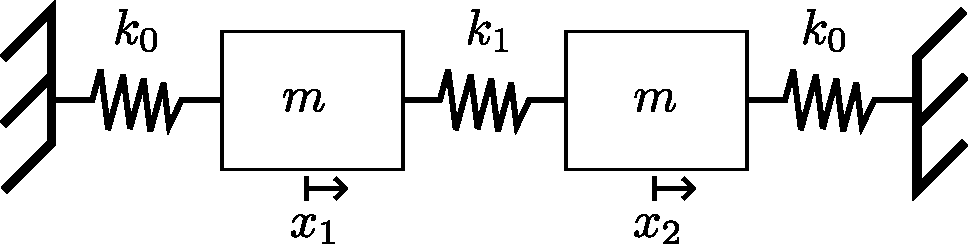
\includegraphics[width=0.4\paperwidth]{figures/coupled-oscillators-diagram}
\par\end{center}

By inspection, the equations of motion are:
\begin{eqnarray}
m\ddot{x}_{1} & = & -k_{0}x_{1}+k_{1}(x_{2}-x_{1})\\
m\ddot{x}_{2} & = & -k_{0}x_{2}-k_{1}(x_{2}-x_{1})
\end{eqnarray}
which may be written in matrix form as
\begin{equation}
\mathbf{\ddot{x}}=\frac{1}{m}\left[\begin{array}{cc}
-(k_{0}+k_{1}) & k_{1}\\
k_{1} & -(k_{0}+k_{1})
\end{array}\right]\mathbf{x}
\end{equation}
Because of the form of the matrix%
\footnote{The matrix $\left[\begin{array}{cc}
a & b\\
b & a
\end{array}\right]$ has eigenvectors $\left(\begin{array}{c}
1\\
1
\end{array}\right)$ and $\left(\begin{array}{c}
1\\
-1
\end{array}\right)$ with eigenvalues $(a+b)$ and $(a-b)$.%
}, we can immediately see that it has eigenvectors corresponding to
common and differential motion, with eigenvalues $\left\{ -k_{0},-(k_{0}+2k_{1})\right\} $. 

Applying this diagonalization, we find:
\[
\mathbf{\ddot{x'}}=\frac{1}{m}\left[\begin{array}{cc}
-k_{0} & 0\\
0 & -(k_{0}+2k_{1})
\end{array}\right]\mathbf{x'}\text{ where }\mathbf{x'}=\left[\begin{array}{cc}
1 & 1\\
1 & -1
\end{array}\right]\mathbf{x}
\]
The presence of the coupling $k_{1}$ only affects the differential
mode.


%% \subsection{Damped oscillators}

%% Now consider a mass connected to the wall via a spring with spring
%% constant $k$ and a velocity damper with damping constant $\gamma$:

%% \begin{center}
%% 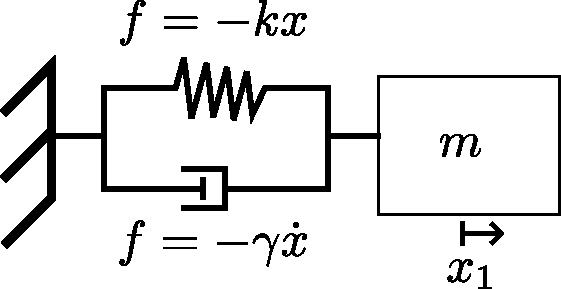
\includegraphics[width=0.25\paperwidth]{figures/damped-oscillator-diagram}
%% \par\end{center}

%% The equation of motion of the mass is:
%% \begin{equation}
%% m\ddot{x}=-kx-\gamma\dot{x}+f_{external}
%% \end{equation}
%% with Laplace transform
%% \begin{equation}
%% ms^{2}X=-kX-\gamma sX+F_{external}
%% \end{equation}
%% giving rise to a transfer function of

%% \begin{eqnarray*}
%% \frac{X}{F} & = & \frac{1}{ms^{2}+\gamma s+k}\\
%%  & = & \left(\frac{1}{m}\right)\frac{1}{\left(s-s_{+}\right)\left(s-s_{-}\right)}\text{ with }s_{\pm}=-\frac{1}{2}\frac{\gamma}{m}\pm\frac{1}{2}\sqrt{\left(\frac{\gamma}{m}\right)^{2}-4\frac{k}{m}}
%% \end{eqnarray*}


%% \subsection{Optical damping}

%% Suppose the cavity mirrors are traveling away from each other with
%% a velocity $v$. Then the phase of the reflected beam is changing
%% at a rate $\left(2\pi/\lambda\right)2v$. We can interpret this as
%% the light being Doppler shifted by $\Delta\omega=\left(2\pi/\lambda\right)2v$.
%% This optical frequency shift will cause the cavity to be closer or
%% further to resonance as compared to a cavity with stationary mirrors.

%% From this we can calculate the optical damping coefficient $\gamma$:

%% \[
%% \gamma\equiv-\frac{\partial f}{\partial v}=-\frac{\partial}{\partial v}\frac{2P}{c}=-\frac{2}{c}\frac{\partial\phi}{\partial v}\frac{\partial P}{\partial\phi}
%% \]
%% where $\frac{\partial\phi}{\partial v}=\frac{\partial\phi}{\partial\omega}\frac{\partial\omega}{\partial v}=\left(1/fsr\right)\left(4\pi/\lambda\right)$
%% so
%% \[
%% \gamma=\frac{2}{c}\frac{1}{fsr}\frac{4\pi}{\lambda}2Fg^{2}\frac{\cos(\phi)\sin(\phi)}{\left(1+F\sin^{2}\phi\right)^{2}}P_{IN}
%% \]

\begin{figure}
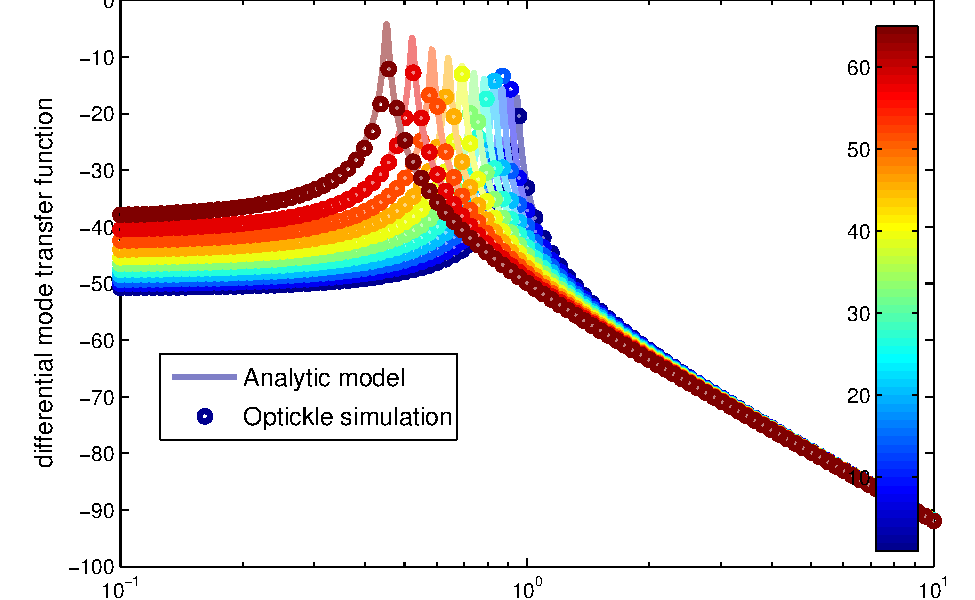
\includegraphics[width=\columnwidth]{figures/model-comparison}
\caption[Optical spring transfer function (numerical and analytic)]{\label{fig:model-comparison}The optical spring effect:  As a cavity is detuned from resonance, the resonance of the differential mode deceases.  This figure compares the resultsof a numerical  (Optickle) model with analytic results. The units of the
  y-axis are $20\log_{10}$(displacement/force); the x-axis is Hz;
  color indicates cavity detuning in picometers.}
\end{figure}

\chapter{Additional Notes}
\label{chapter7}
\section{The Jacobi-Anger Identity}
\label{sec:jacobi-anger}
Taking the generating function of the Bessel functions
\begin{equation}
\exp\left\{\frac{1}{2} z \left(t - t^{-1}\right)\right\} = \sum_{m=-\infty}^\infty t^m J_m(z)
\end{equation}
we can make the substitution $t = \exp \{i \omega t'\}$.
This gives the Jacobi-Anger expansions, which are useful for expanding sinusoidal phase modulation in terms of sidebands around the carrier:
\begin{align}
e^{i\Gamma\cos\Omega t} & = \sum_{n=-\infty}^{\infty} \left(i^n\right)  J_n(\Gamma) \exp\{i n \Omega t\} \\
e^{i\Gamma\sin\Omega t} & = \sum_{n=-\infty}^{\infty} J_n(\Gamma) \exp\{i n \Omega t\}
\end{align}

\section{Comparison of Phase Modulation (PM) and Amplitude Modulation AM)}
\label{sec:am-vs-pm}
%
Suppose we have a signal consisting of a carrier (at frequency $\omega$ and
with unit amplitude) and two sidebands, of amplitudes $a$ (lower) and $b$
(upper), separated from the carrier by a frequency $\Omega$:
%
\begin{equation}
E(t) = \left(1 + a \exp(-i \Omega t) + b \exp(i \Omega t)\right)
\exp(i \omega t)
\end{equation}
%
To find the power in this signal, we take the
modulus squared, $P = E^*E$ where * is the complex conjugate:
%
\begin{equation}
\begin{split}
P = & \left(1 + |a|^2 + |b|^2\right) \\
    & + \left(a^* + b\right) \exp(-i \Omega t) + \left(a + b^*\right) \exp(i \Omega t) \\
    & + \left(ab^*\right) \exp(-2 i \Omega t) + \left(a^*b\right) \exp(2 i \Omega t)
\end{split}
\end{equation}
%
The condition for the $1\Omega$ variation in the power to vanish is
$a=-b*$, i.e. the real parts of the amplitudes of the sidebands must
be opposite, and the imaginary parts must be equal. So we can extract
the amplitude and phase modulation indicies:
%
\begin{equation}
\begin{split}
m_{AM} &= (a + b^*)\\
m_{PM} &= (a - b^*)
\end{split}
\end{equation}

What is the condition for the $2\Omega$ signal to vanish? With just
two sidebands, it will always be present (though at second order in
the sideband amplitude). In true phase modulation, the $2\Omega$
signal is cancelled by the interaction of (the infinite number of)
higher-order sidebands. As best I can tell, there is no simple
arrangement of this cancellation other than via a magical property of
the Bessel functions.

\section{Comparison of Phase Modulation (PM) and Frequency Modulation (FM)}
There is not really any difference between phase modulation and frequency modulation.
Frequency modulation with modulation depth $m_{\text{FM}}$
{[}Hz{]} at a frequency $f$ {[}Hz{]} has the form
\begin{align}
y(t) &=\exp\left\{ i\omega t\right\} \exp\left\{ i\int_{0}^{t}2\pi\ m_{\text{FM}}\ \Re\left\{ e^{i2\pi ft'}\right\} \ dt'\right\} 
\intertext{where $\omega$ [radians/second] is the carrier frequency. We
can simply do the integral and get:}
y(t) &=\exp\left\{ i\omega t\right\} \exp\left\{ i\ \frac{1}{f}\ m_{\text{FM}}\ \Re\left\{ ie^{i2\pi ft}\right\} \right\} 
\end{align}
which is just phase modulation at frequency $f$ {[}Hz{]} with modulation
depth $(i/f)m_\text{FM}$ (in radians).
%\[
%\frac{d}{dt}\left(\frac{1}{f}m_{\text{FM}}\sin2\pi ft\right)=2\pi\ m_{FM}\cos2\pi ft
%\]
The relation between phase modulation and frequency modulation is therefore:
\[
m_{\text{PM}}=\left(\frac{i}{f}\right)m_{\text{FM}}
\]
The $i$ signifies a phase shift of 90 degrees in the modulation (turning
$\cos$ to $\sin$).



\begin{comment}
\section{Displaced and Misaligned Beams}

References to cite: \cite{Anderson1984Alignment,Hauck1980Misalignment}.
\end{comment}
\section{Calibration}

The calibration of the LIGO interferometers into real units (of mirror
displacement or gravitational wave strain) during Initial LIGO is
described in~\cite{KisselCalibrationPaper}; the Enhanced LIGO procedure
was essentially the same.  An alternate calibration procedure using
radiation pressure is described in \cite{Goetz2010Gravitational}.

\section{Only the Signal Field Matters}

Suppose we have two electric fields incident on a photodiode: the
signal field $A_s$ and the local oscillator field $A_{LO}$.  The power
seen by the photodiode is
$$ \left| A_s + A_{LO} \right|^2 = 
   |A_s|^2 + |A_{LO}|^2 + 2 \mathrm{ Re } {A_s}^*A_{LO}$$
In the small-signal regime, $|A_s| << |A_{LO}|$.  The signal on the
photodiode is proportional to $A_s A_{LO}$ while the shot noise is
proportional to $\sqrt{|A_s|^2+|A_{LO}|^2}\approx A_{LO}$.  
  The detected SNR is independent of the local oscillator strength.

\section{Optical Phase Conventions}

In writing down the relationships between optical field amplitudes
upon reflection from or transmission through a mirror, we must first
choose a phase convention. What happens to the phase of the field upon
reflection? Upon transmission? For a real mirror, made up of many
layers of dielectric coating on both sides of a thick substrate, and
given particular reference points at which to compute the fields, the
phases upon reflection and transmission depend on all of this
structure. But for tractability, and for no real loss of modeling
fidelity, we can discard the particulars as unknown `microscopic
phase' and adopt instead an idealized model of a mirror that has the
right power reflectivity and transmission and does not violate
conservation of energy. There are two such conventions in common
use. We can call them the ``engineers' convention'' and the
``physicists' convention.''

\begin{figure}
\centerline{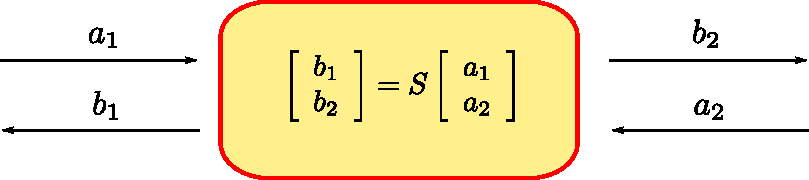
\includegraphics{figures/Smatrix.pdf}}
\caption[Scattering matrix]{\label{fig:Smatrix}The scattering matrix $S$ 
gives the amplitudes of the outgoing fields $b_1$ and $b_2$ in terms of
the in-going fields $a_1$ and $a_2$.}
\end{figure}

The complex reflection and transmission coefficients are encoded in
the S-matrix, which gives the amplitudes of the fields going
\emph{out} of some optical element in terms of the fields going
\emph{in} (depicted in figure~\ref{fig:Smatrix}).

In the physics convention, transmission through a mirror conveys no
phase; reflection from one direction is real and positive ($+r$),
but reflection from the other direction gives a minus sign ($-r$).
The physics convention essentially models a mirror as a single dielectric
boundary.  The S-matrix for the physics convention is:
%
\begin{equation}
S_{physics}=\left(\begin{array}{cc}
-r & t\\
 t & r
\end{array}\right)
\label{eq:Smatrix-physics}
\end{equation}

In the engineering convention, reflection from either side of a mirror
has the same real, positive reflectivity ($+r$), but transmission
through the mirror gives a phase of 90 degrees, a coefficient of $it$, 
giving an $S$-matrix of:
%
\begin{equation}
S_{engineering}=\left(\begin{array}{cc}
 r & it\\
it & r
\end{array}\right)
\label{eq:Smatrix-engr}
\end{equation}

The (initial) LIGO test masses actually have amplitude reflectivity
coefficients close to $-1$ at the high-reflectivity (HR) side, so
that the electric field on the surface of the optic on the high-power
side is very near zero.%

\section{Gaussian Beams}

The general picture of Gaussian beams is shown here:

It is convenient to introduce the complex beam parameter $q$.  In terms of $q$:
\begin{equation}
\frac{1}{q(z)} = \frac{1}{R(z)} - i \frac{\lambda}{\pi w^2(z)}
\end{equation}
where $R(z)$ is the radius of curvature of the phase fronts at a
position $z$ along the optical axis, and $w(z)$ is the spot size at
that location.  We can also write:
$q(z) = i z_R + (z - z_0)$.

For a mode to resonate in an optical cavity, the spherical surface of
the mirrors must match the spherical phase front of the beam at the
location of the mirror.

Suppose mirror 1 has curvature $R_1$ and coordinate $z_1$, and
similarly for mirror 2.  We would like to solve for the waist location
and Rayleigh range.

References: Kogelnik and Li \cite{Kogelnik1966Laser}, Siegman \cite{Siegman1990Lasers}, \cite{Rudiger1998Phase,Fox1961Resonant}.

\section{Laser Modes}

The eigenmodes of an optical cavity formed from spherical lenses are
the Hermite-Gauss (if the cavity has rectangular symmetry) or
Laguerre-Gauss (for axial symmetry) modes.  The amplitude distribution
at the beam waist is a Gaussian multiplied by a Hermite or Laguerre
polynomial.  These are exactly the same familes of functions as the
energy eigenstate wavefunctions of the simple harmonic oscillator in
quantum mechanics.

\begin{comment}
\section{Feedback Control}

Operation of the LIGO detectors relies crucially on feedback control
systems.  In general, the response of the optical plant is completely
nonlinear; in order to produce a valid readout, the plant must be held
very close to its operating point.  The use of feedback control allows
us to attain linear response from an otherwise very nonlinear machine.

Here is a basic diagram of a feedback system:

Algebraically, one can derive a relationship giving the transfer function
of the closed-loop system in the Laplace domain:
\end{comment}

\begin{comment}
\section{The Antenna Pattern and the Free Spectral Range (FSR)}
\label{sec:antenna-pattern}
Gravitational waves come in two polarizations; for waves impinging
from a given direction, the second polarization represents an ellipse
of oscillating transverse strains rotated 45 degrees relative to the
first.  

Fundamentally, a Michelson interferometer is sensitive to two
polarizations of gravitational waves.  However, as discussed in chapter~\ref{chapter2}, we
elect to throw away sensitivity to one polarization in return for
common-mode noise immunity in the second polarization.

Although the waves come in two polarizations, one should note that
there is no globally consistent notion of \emph{the} $h_+$ and
$h_\times$ polarizations.  This is forbidden by the Hairy Ball
theorem.  

For a single detector, we can identify $h_+$ as the polarization
that shows up in DARM, and $h_\times$ as the polarization that would
show up in CARM.  Immediately (again due to the hairy ball theorem) we
see that there must be nulls in the sensitivity pattern of a single
interferometer.

In section~\ref{sec:long-wavelength}, we introduced the \emph{long
  wavelength approximation}, in which we assume that the gravitational
wave phase changes slowly compared to the time required for light to
travel from one end of an interferometer arm to the other end.  This
approximation holds in the LIGO detection band ($f \lesssim 7000$ Hz
corresponds to $\lambda \gtrsim 40$ km) but fails completely for GW
frequencies equal to the free spectral range of the arm cavities,
where the GW wavelength exactly matches the arm length.  For a
normally incident GW at this frequency, a photon traversing the arm
will see an elongated optical path length on its trip down the arm but
a contracted path length on its return trip, yielding zero net effect.
The antenna pattern is therefore a frequency-dependent function; to
calculate it, we must consider the spatial extent and time evolution
of the gravitational wave.

%% FIXME: References to cite:
%% \cite{Giampanis2008Search,Schilling1997Angular,Rakhmanov2008Highfrequency,Butler2004Characterization,Fricke2007HighFrequency}
\end{comment}
\section{Shot Noise}
The root-mean-square of a Poisson process with current $I$ and quantum
$q$ measured over a bandwidth of $\Delta f$ is 
$$\sigma = \sqrt{2 q I \Delta f}$$ 
Here $I$ could be the electric current in Amps (=Coulombs/second) and
$q$ the charge of an electron.  For light incident on a photodiode,
the photon shot noise can be considered as an energy current, with
$I\leftarrow P$ being the DC power, and $q\leftarrow h\nu$ being the
energy per photon.

The amplitude spectral density of this process is white, with
amplitude $\sqrt{2qI}$ in units of [I] per square root of Hz.
For power $P$, the shot noise amplitude spectral density is 
\begin{equation}
\text{shot noise ASD} = \sqrt{2 h\nu P}\quad [\text{Watts}/\sqrt{\text{Hz}]}
\label{eq:shotnoise-asd}
\end{equation}
which gives a relative intensity noise of $\sqrt{2 h\nu/P}$.

\begin{comment}
\section{Noise analysis of opamp circuits}

\begin{figure}
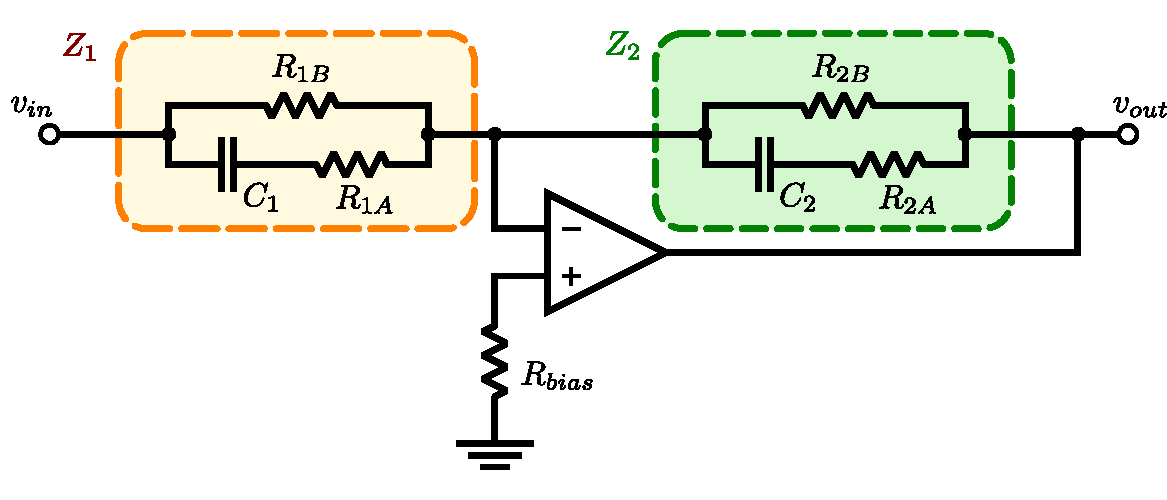
\includegraphics[width=\columnwidth]{notes/figures/inverting-amp.pdf}
\caption{\label{fig:inverting-amp}Basic active filter in the inverting amplifier configuration.} 
\end{figure}

Cite: Art of Electronics\cite{ArtOfElectronics}
\end{comment}
%\cite{Quetschke2007Complex}
%\cite{Williams1972Optics}


\singlespace
\bibliographystyle{plain}
\bibliography{tobin}


\singlespace
\chapter*{Vita}

Tobin Fricke was born in Los Angeles, California in 1980 to Oscar and
Julie Fricke.  After graduating from Mission Viejo High School in
1998, he studied electrical engineering and computer science (EECS)
and mathematics at the University of California, Berkeley and physics
at the University of Rochester.  Following his doctoral work at
Louisiana State University, Tobin will begin an appointment at the Max
Planck Institute for Gravitational Physics in Hannover, Germany.


\end{document}
